\documentclass[a4paper]{article}

\usepackage[utf8]{inputenc}
\usepackage[T1]{fontenc}
\usepackage{%
    amsmath,
    amssymb,
    graphicx,
    xspace,
    subcaption
}

\graphicspath{{../imgs/}}

\newcommand \rmin[1][]      {\ensuremath {r^{#1}_{\min}}\xspace}
\newcommand \rmax[1][]      {\ensuremath {r^{#1}_{\max}}\xspace}
\newcommand \region[1][]    {\ensuremath {(\rmin[#1], \rmax[#1])}\xspace}
\newcommand \state[1][]     {\ensuremath {s^{#1}}\xspace}
\newcommand \currstate      {\ensuremath {\state[t]}\xspace}
\newcommand \nextstate      {\ensuremath {\state[t+1]}\xspace}

\title{%
    CARPET: Coarse Action Reinforcement Policy Extraction Tool
}

\author{%
    Andreas Holck Høeg-Petersen
}

\begin{document}

\maketitle

\noindent
We start by creating a partitioning based on a select set of predicates over the
state space. Then we use a dataset $D$ of observations of state-action pairs
from $n$ trajectories of the environment\footnote{In this setup $n=100$ and the
    well-trained agent reaches 400 timesteps in each run resulting in $|D| =
400000$} to split those regions where the agent will either choose action 0 (`no
hit') or action 1 (`hit'). This is done using polynomial logistic regression
with each observed state being labelled according to the action associated with
it. The degree of the polynomial is chosen by starting with simple linear
regression (ie.\ degree 1) and repeating the regression with an incremented
degree if the accuracy of the split is lower than 0.95.

\begin{figure}[ht]
    \centering
    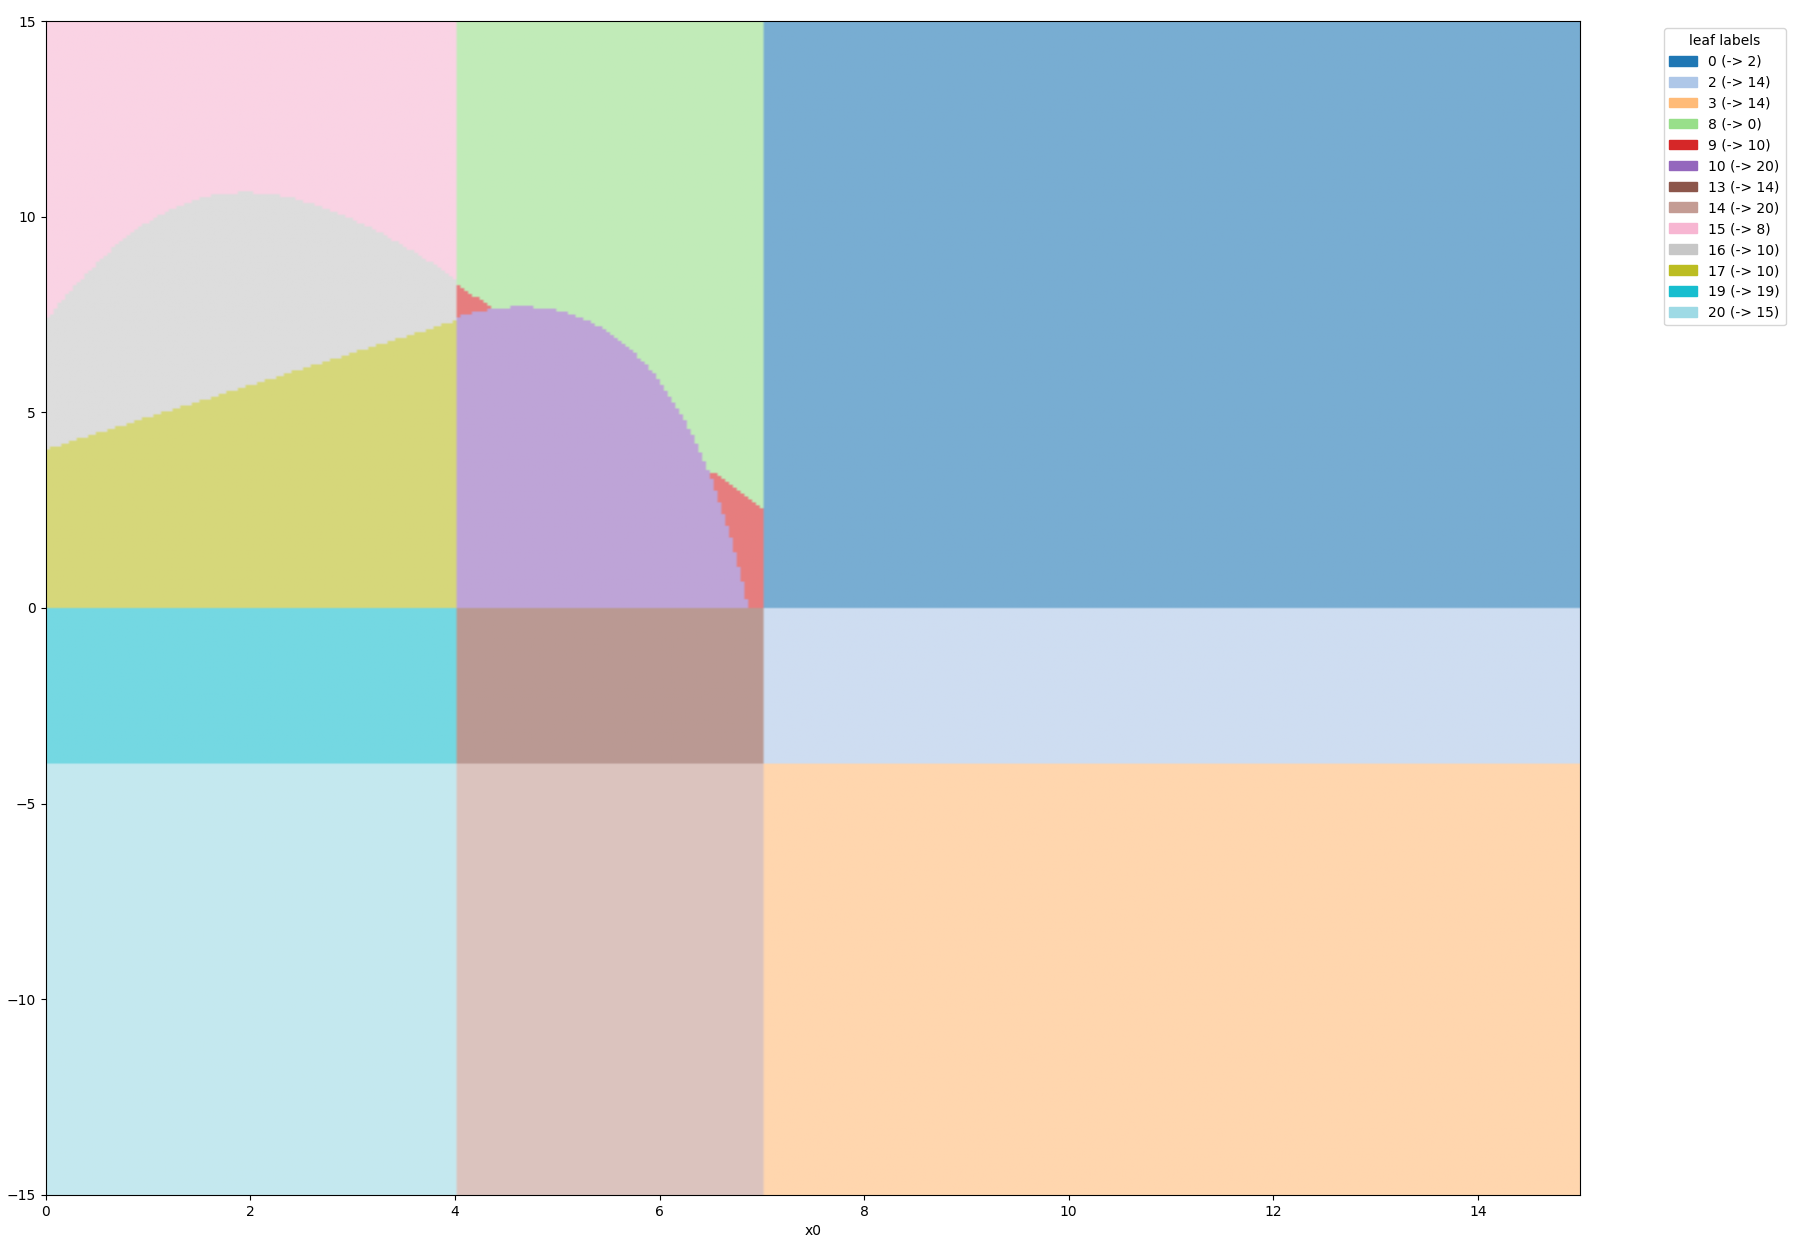
\includegraphics[width=.9\textwidth]{initial-action-split}
    \caption{%
        State space partitioning after splitting according to action. The
        axis-aligned splits are based on the initial predicates, the other are
        based on polynomial regression to separate regions based on the action
        performed.  Regions in this figure are not labelled with their
        corresponding action, but uniquely colored. The legends shows what the
        most likely next region is from each region.
    }
    \label{fig:initial-split}
\end{figure}

Figure~\ref{fig:initial-split} shows the emerging regions in different colors.
Furthermore, we use $D$ to estimate the next-region transitions for each region.
That is, for each region $\nu_i$ we observe a set of states $S_{\nu_i} \subseteq D$
that fall within that region. Let $s_{j,t} \in S_{\nu}$ be the state we
encountered in the $j$th trajectory at timestep $t$. For each state $s_{j,t} \in
S_{\nu_i}$ we check what region $s_{j,t+1}$ belongs to and a get a next-region
transition probability estimate based on $D$.

Assessing the quality of this model is done by simply executing the environment
again and now comparing the predicted next regions with the actual next region.
In that case, this initial version as an accuracy of 0.69 (for action prediction
the accuracy is 0.99).

Now we try to refine the model by splitting regions according to the next-region
transitions of its states using a fresh dataset $D$. If the states in
$S_{\nu_1}$ transitions to more than 1 other state, we first search for a split
that separates states going to the most common next-region from all the rest and
then we repeat recursively in the new regions.\footnote{As I am writing this, I
    am thinking, that maybe we should start by separating the states that go
    from region $\nu$ to $\nu$ (ie.\ stay within the same region), so that we
don't mess up the structure?} By that process, we go from 21 to 37 regions and
we increase the accuracy to 0.73.

\begin{figure}[ht]
    \centering
    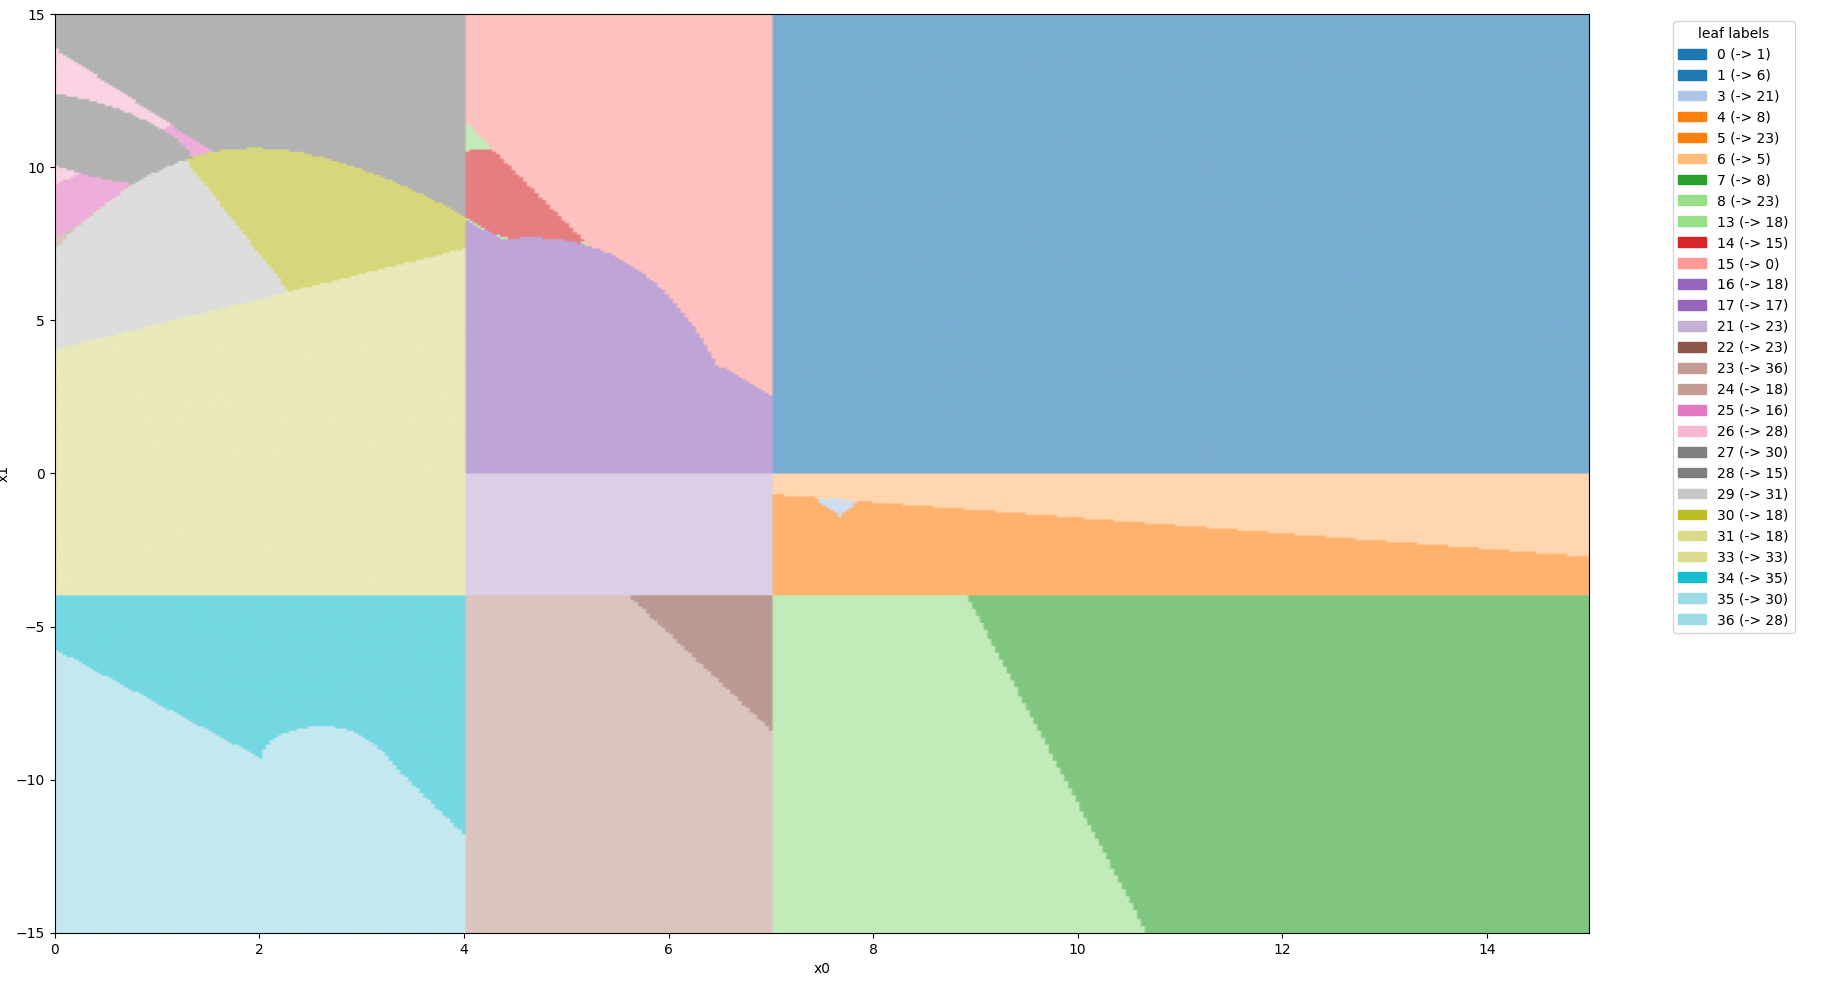
\includegraphics[width=.9\textwidth]{split-round1}
    \caption{%
        The partitioning after the first round of refinement. Note that the
        color map cannot represent all the regions with distinct colors, making
        the interpretation less obvious.
    }
    \label{fig:split-round1}
\end{figure}

We can repeat this process to get a higher precision but increasing the number
of regions even more. In Figure~\ref{fig:split-round2} we see the partitioning
after the second round of next-region based splits, where the partitioning
contains 71 regions and incurs an accuracy of 0.77. However, the splits are
becoming increasingly complicated (that is, more regions are split according to
high-degree polynomial) and for several regions the split is based on very few
data points. Repeating the splitting process after this second round does not
yield any noticable improvements in accuracy, but amplifies the aforementioned
problems.

\begin{figure}[ht]
    \centering
    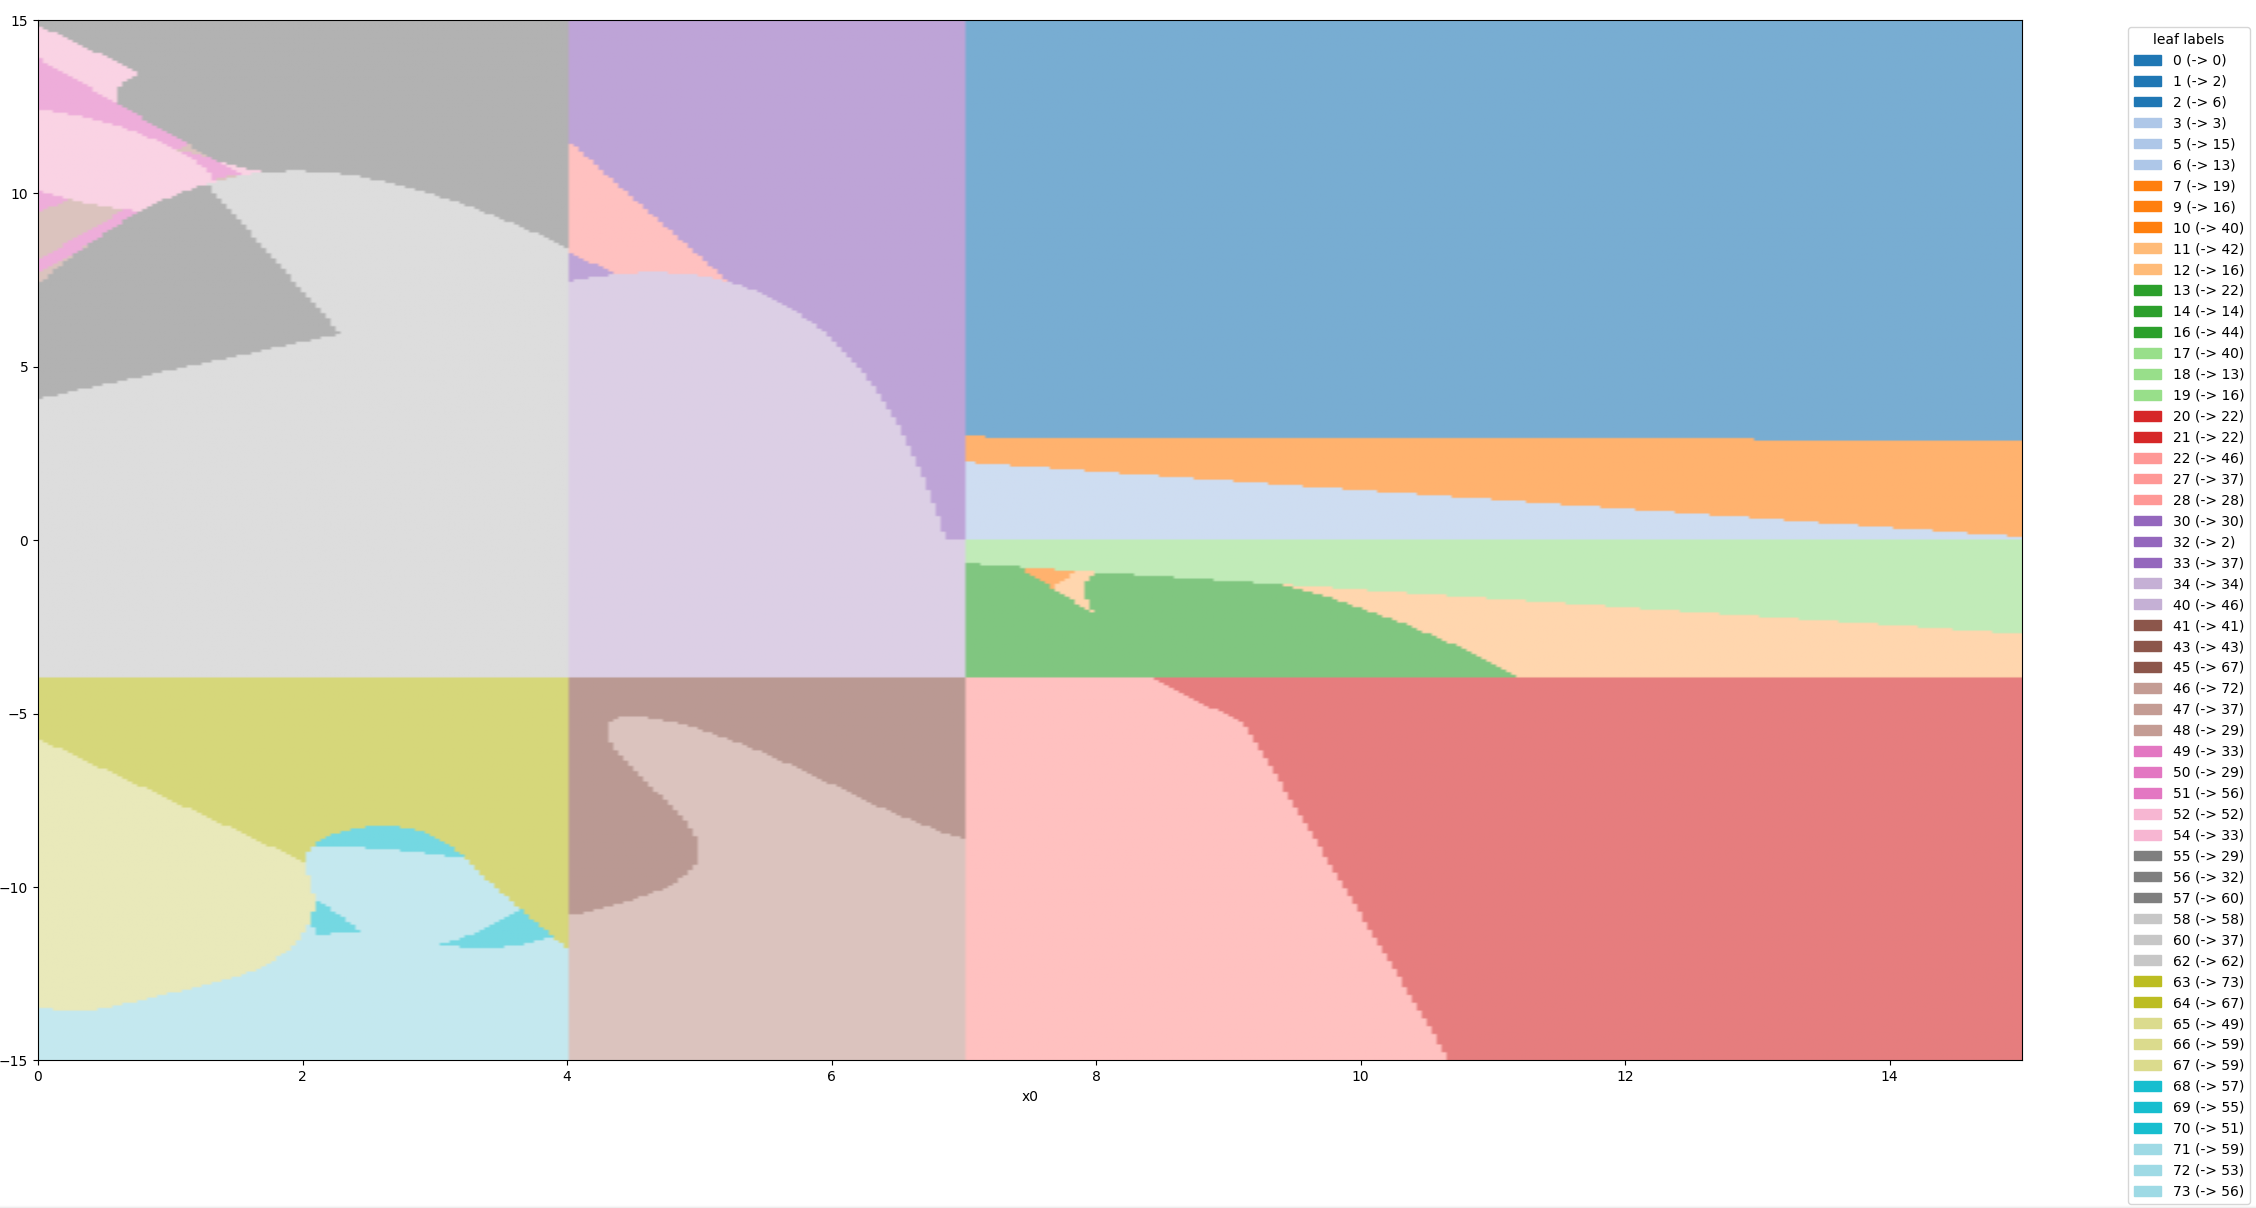
\includegraphics[width=.9\textwidth]{split-round2}
    \caption{%
        The partitioning after the second round of refinement. The legend is now
        no longer able to show all the regions.
    }
    \label{fig:split-round2}
\end{figure}

Another problem occurs in the regions where the next-region transition is
stochastic. For the very coarse original partitioning (in this particular
example), we observed no stochasticity in the transitions. But as the
partitioning is refined, regions appear where states can transition to mulitple
different regions dependent only on unknown randomness, thus making a clean
split impossible.

In Figure~\ref{fig:inaccuracy} we show an example of this. The colored stripes
represent regions where as the small crosses represent observed states. The
color of the crosses indicate what region that state transitions to at the next
state. Note that these states and transitions are sampled from actual executions
of the environment and the transitions are not deterministic. We do see some
pattern in the transitions, but it is also clear that it is impossible to do a
perfect split. Thus, we need to come up with a different approach.

\begin{figure}[ht]
    \centering
    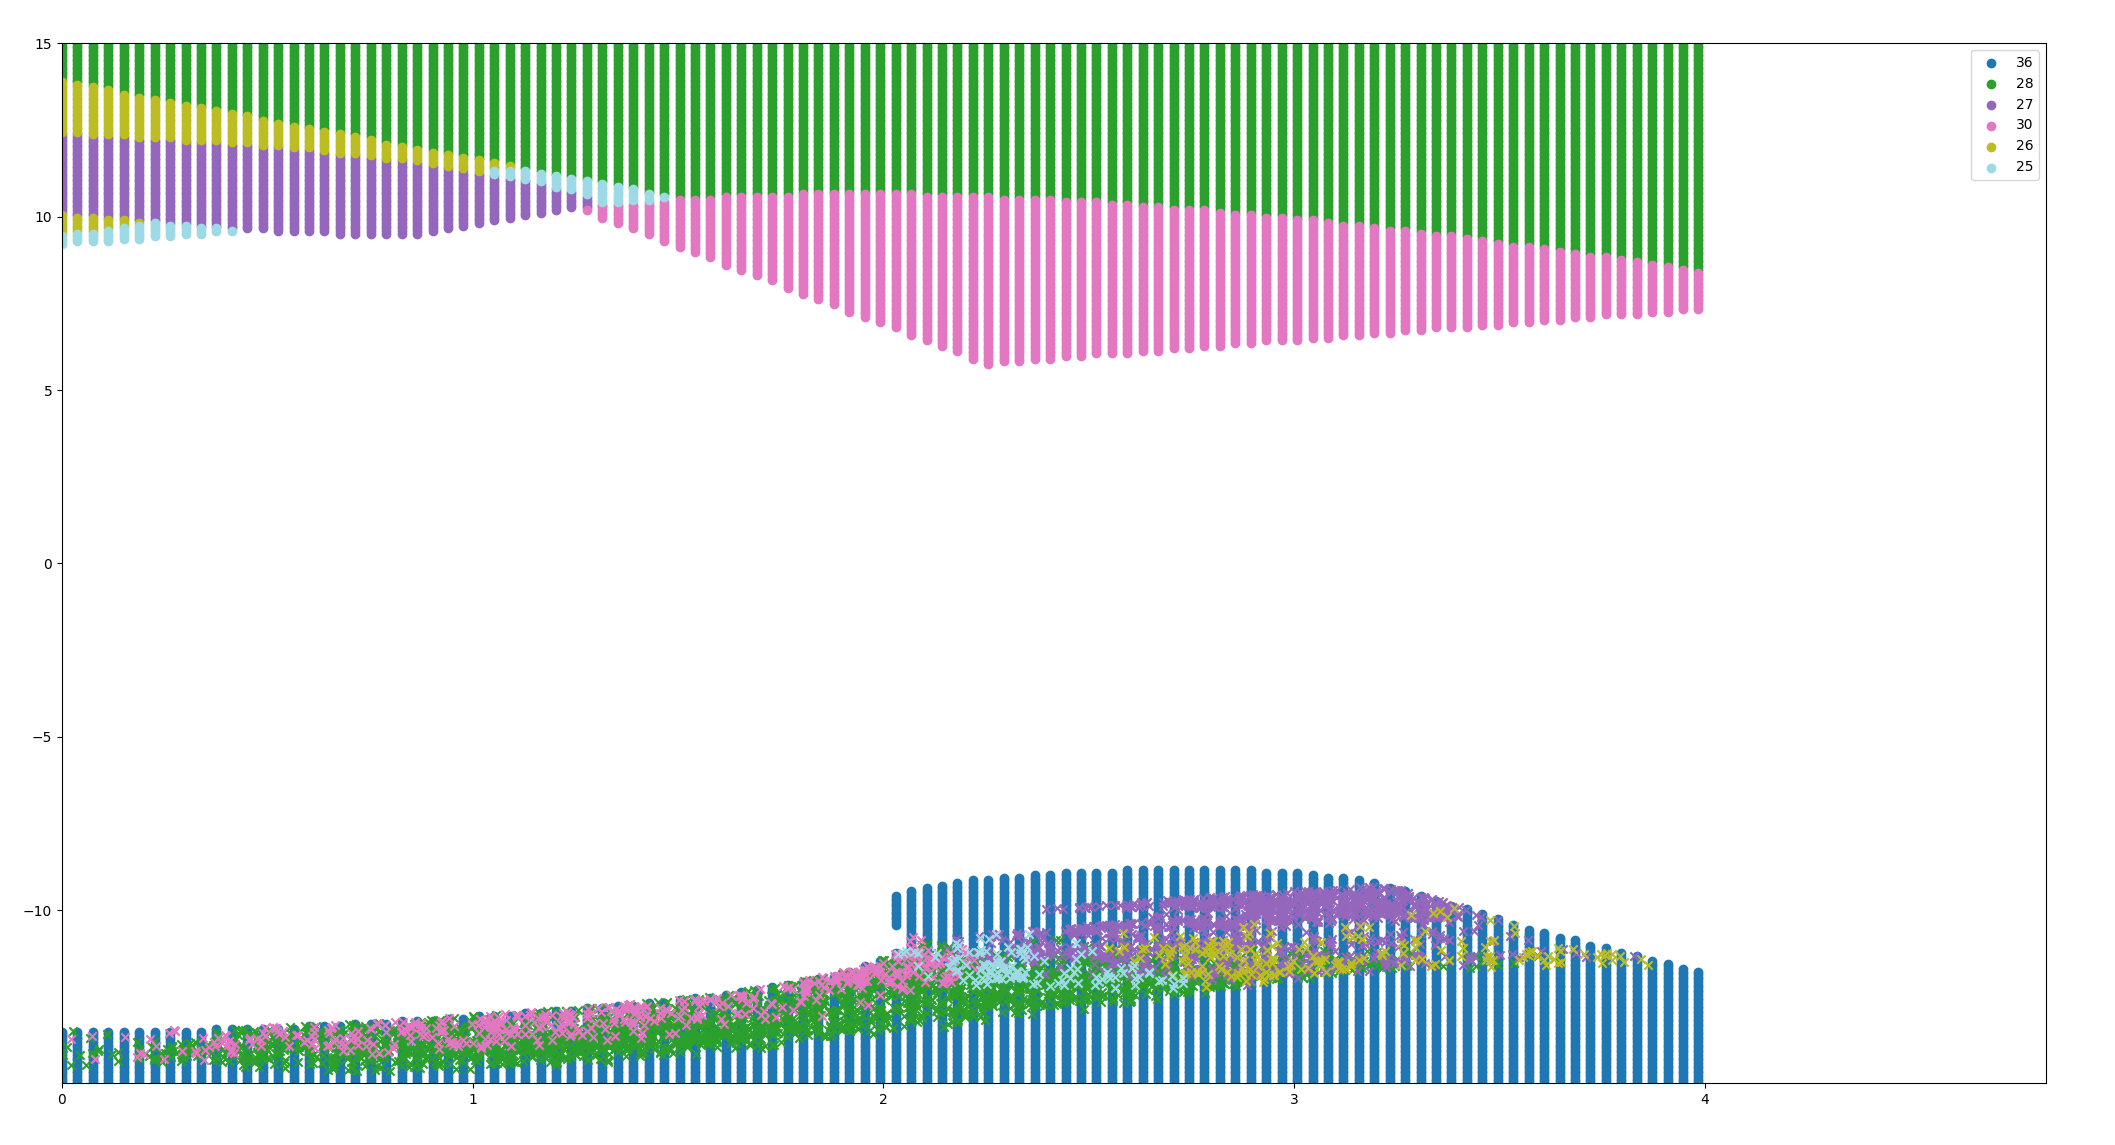
\includegraphics[width=.9\textwidth]{inaccuracy-1}
    \caption{%
        A closer look at the states (the colored crosses) in a given region (the
        blue striped area) and the regions that the states transitions to in our
        sampling data (the color of a cross correspond to the color of the
        striped region it will transition to).
    }
    \label{fig:inaccuracy}
\end{figure}

One approach that we have discussed earlier is to characterize each state by the
probability distribution of its next-region transition. This would require that
we take each observed state (or we sample states systematically or randomly) and
then sample adequately many next-states to get a sample distribution of the
next-region transition probability. We would then need to learn a mapping from a
state to a probability distribution and then do our split according to this.

\subsection{Checking for next actions}%
\label{sec:next-action}

These next images show some instances where the next regions of a state is a
`hit'-state. Here, my idea have been to make splits according to the future
actions, so in that way predict the future behavior. I have not yet implemented
splits on this condition, but nonetheless, it might be interesting.

\begin{figure}[ht]
    \centering
    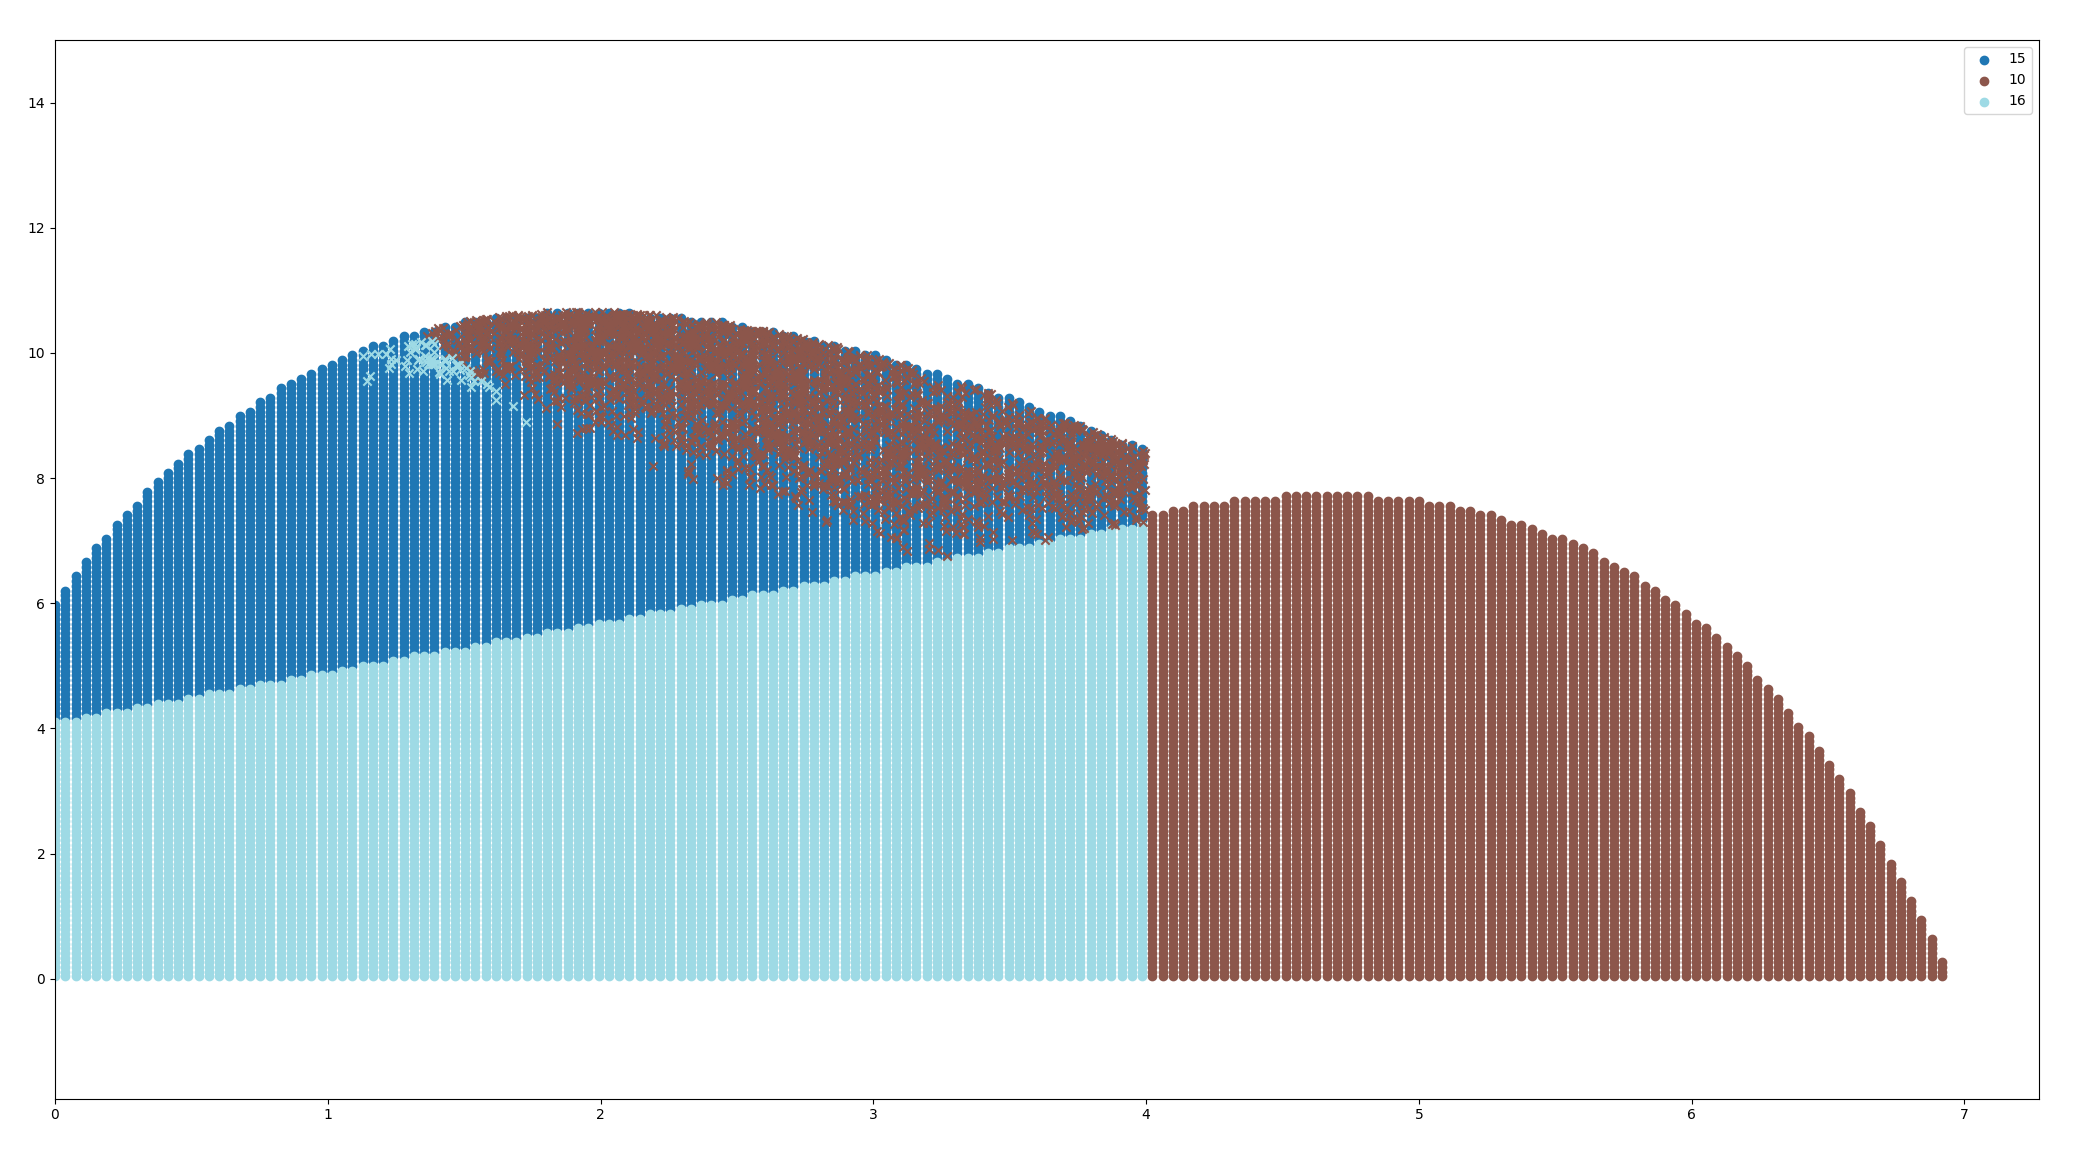
\includegraphics[width=.9\textwidth]{hit-next-2a}
    \caption{%
        In the blue region, the brown crosses will go to the brown state, where
        the action is `hit'. The light-blue crosses will go to the light-blue state.
    }
    \label{fig:hit-next-2a}
\end{figure}


\section{Clustering and Total Variational Distance}

In this section, we look at using agglomorative clustering to come up with
region splits. We also use Total Variational Distance (TV) to assess the quality
of a split. As the splitting procedure begins, the TV distance is at 1 every
time. When we encounter lower values, we inspect that further (see below).
First, we take a look at some unwanted behavior earlier.

In Figure~\ref{fig:seperation-sketchy} we see a region whose points are
separated into 2 clusters (red and pink), which is to be used as the basis for
splitting the region in 2. While the pink cluster seems fairly coherent, the
red points are scattered in 2 different locations. One that seem to have a
natural separation border with the pink cluster, and another along the border of
the region itself, lumped in with the pink points.

\begin{figure}[ht]
    \centering
    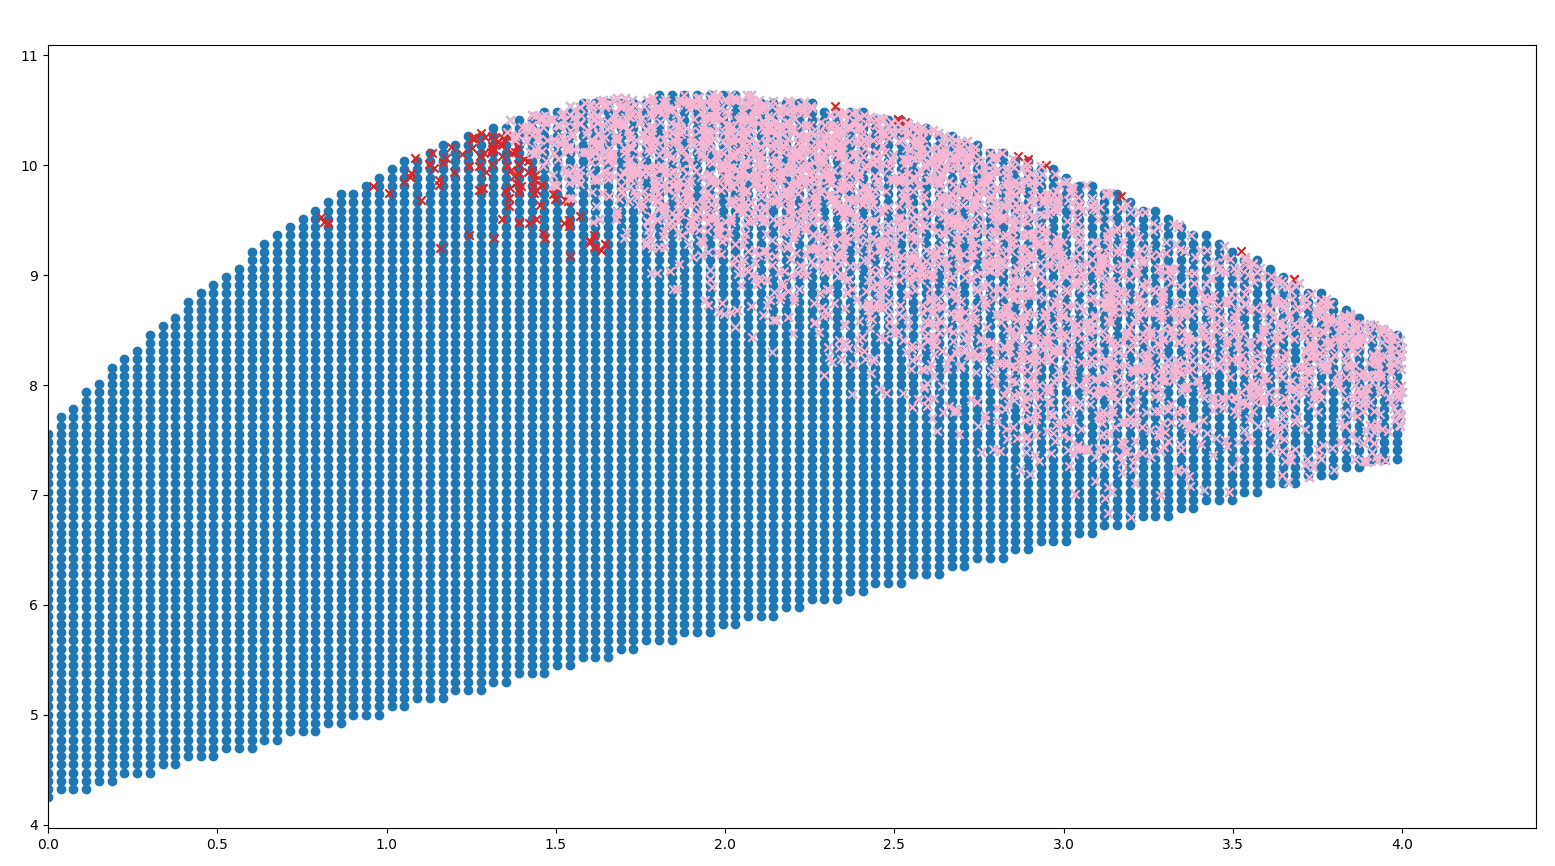
\includegraphics[width=0.8\textwidth]{seperation-sketchy}
    \caption{All the pink crosses transitions to the same region. The red ones
    have 3 different possible regions to go to. Especially, notice the ones in
the top `right' following the edge of the region boundary.}
    \label{fig:seperation-sketchy}
\end{figure}

Upon further inspection, we see that the pink cluster is deterministic in its
transition probability, that is, all points transition to the same next region
(region 10).  The red cluster, however, transitions to 3 different regions. The
points spread along region border (together with the pink points) all transition
to region 8, while the rest go to either region 17 (predominantly) or 16.

The \textbf{question becomes}: how can we make a separation that makes the new
regions convex? In this example, the few red points among the pink ones would be
better to include in the pink cluster even though they `pollute' the transition
probaility a little bit.

Another example of conflicting clusters within a region is given in
Figure~\ref{fig:misclassification}. This is a result of the decision boundary
created in an earlier iteration not being perfect --- which is impossible to
achieve. This region should therefore not be split anymore. But, \textbf{how do
we recognise this situation and choose not to split?}

\begin{figure}[ht]
    \centering
    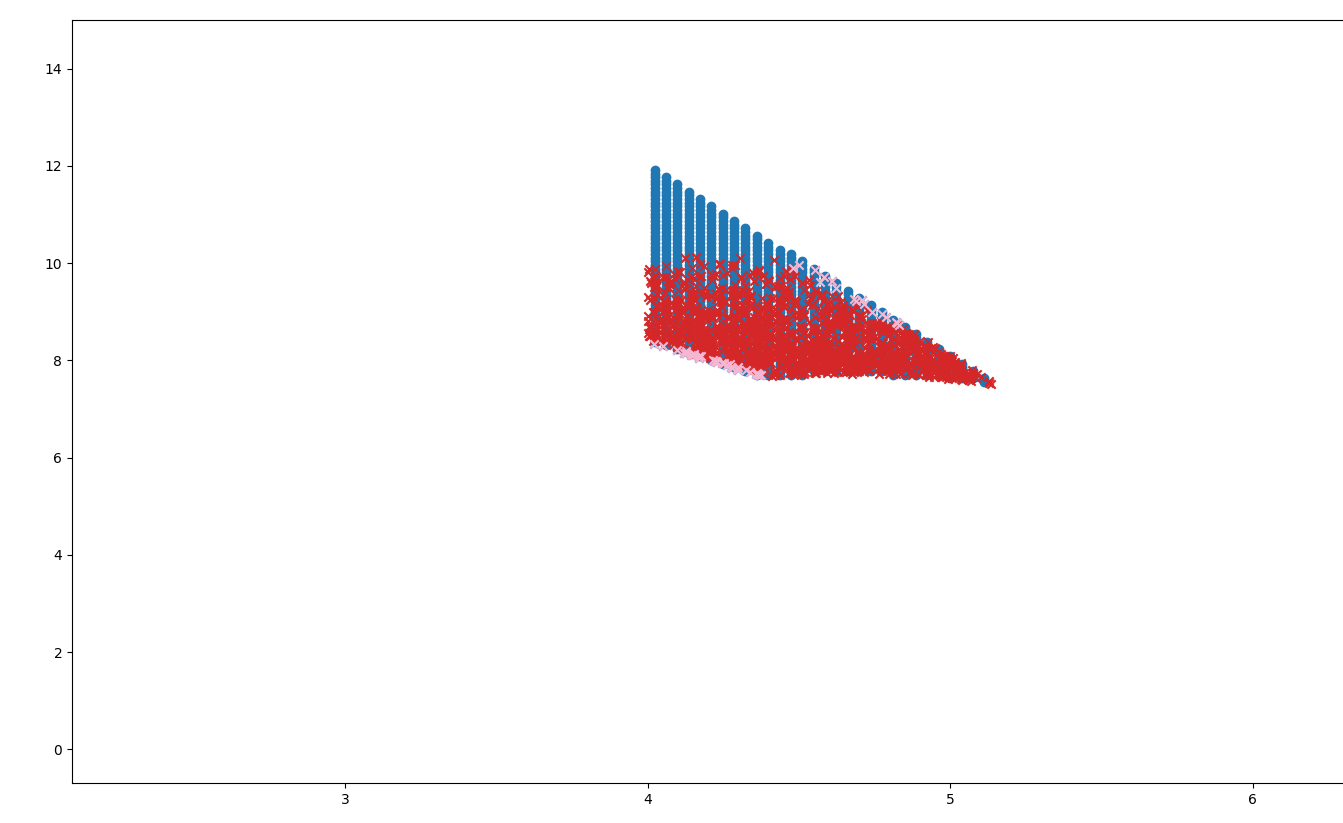
\includegraphics[width=0.8\textwidth]{misclassification}
    \caption{%
        In this example, the red points represent the intended points for this
        region, ie.\ this region is supposed to describe an area, where all
        states transition to the region that the red points go to. The pink
        points are a result of inevitable misclassification during the last
        split and actually belong to neighbouring regions. Therefore, this
        region should not be split any further.
    }
    \label{fig:misclassification}
\end{figure}

\paragraph{Low td value}

In the Figure~\ref{fig:separation-low-td-val}, we also see a non-convex cluster
(the red one) but furthermore, we see that the Total Variational Distance
between the two clusters (measured as the TV distance between the probability
vectors associated with the points in the cluster) is lower than 1.

\begin{figure}[ht]
    \centering
    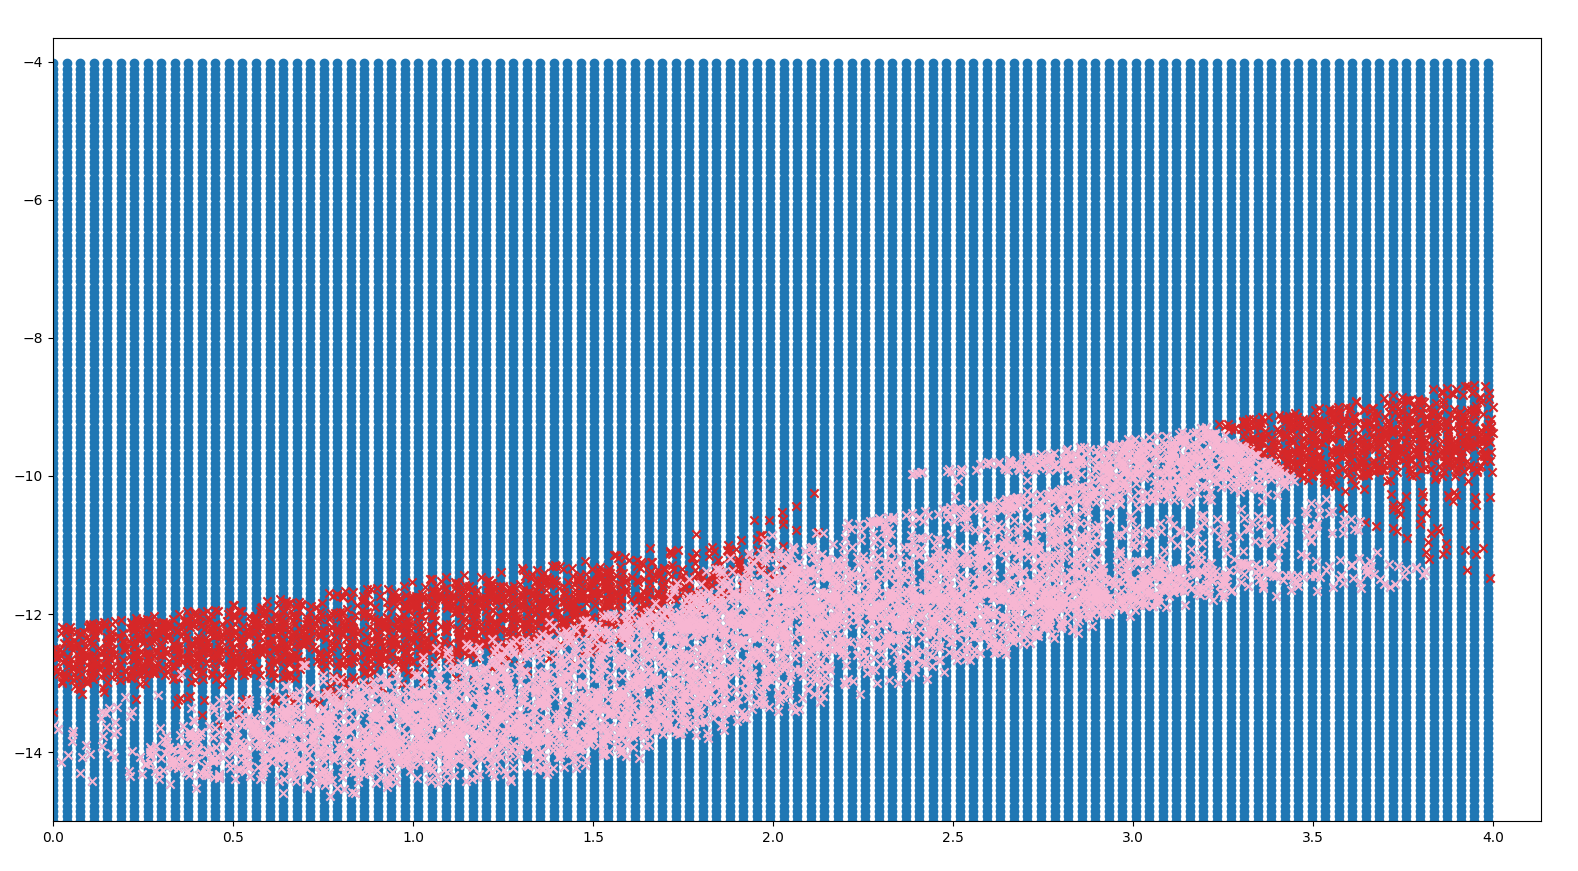
\includegraphics[width=0.8\textwidth]{separation-low-td-val}
    \caption{separation-low-td-val}
    \label{fig:separation-low-td-val}
\end{figure}

By closer inspection it is also seen, that within both groups some states have a
most likely transition to state 16. In previous splits, no such overlap have
happened. This is most likely because the transitions from this region has a
stochastic component --- how much `bounce' happens when the ball hits the ground
(position gets to zero and velocity goes from negative to positive).

We can zoom in to find that the red points with the higher x-value can actually
be perfectly separated from the pink points. However, the other part of the red
cluster overlaps with the pink cluster, see
Figure~\ref{fig:separation-low-td-val-zoom}.

\begin{figure}[ht]
    \centering
    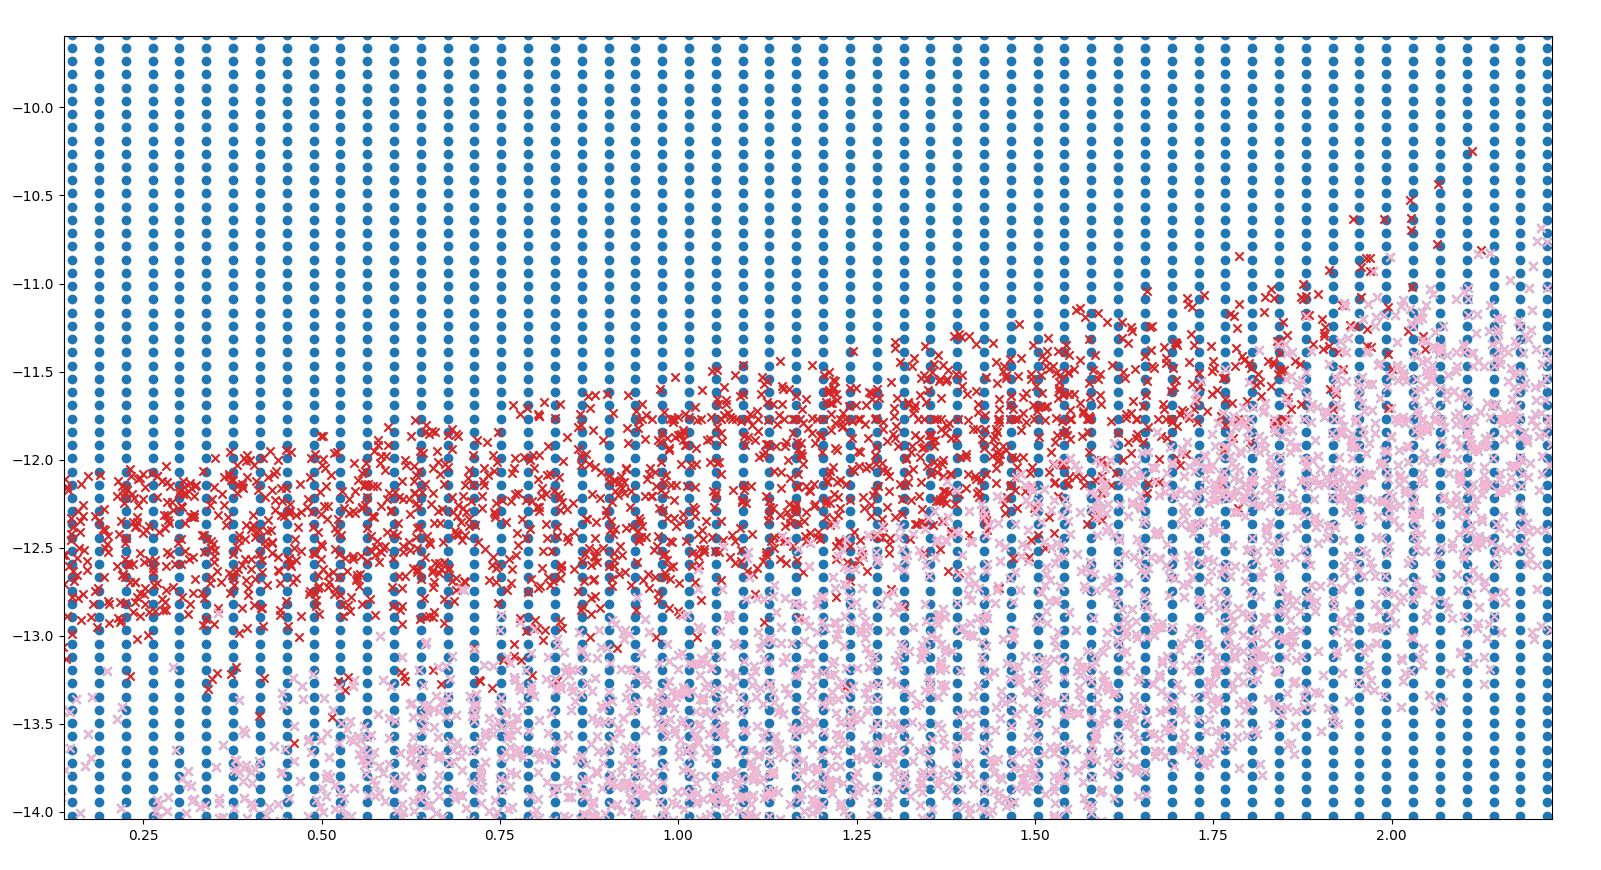
\includegraphics[width=0.8\textwidth]{separation-low-td-val-zoom}
    \caption{separation-low-td-val-zoom}
    \label{fig:separation-low-td-val-zoom}
\end{figure}

By letting the clustering algorithm find 3 clusters instead of 2, we get 2
clusters, call them $a$ and $b$, that each has a single `most likely' transition
(to region 16 and 20, respectively). The third, call it $c$, has states that
most likely transitions to region 15 and others that transition to region 16.
The TD value between $a$ and $b$ are 0.99, and so is it between $b$ and $c$
which don't share any most likely next region. However, between $a$ and $c$ the
TD value is only 0.77. Figure~\ref{fig:separation-low-td-3-clusters} shows this
separation.

\begin{figure}[ht]
    \centering
    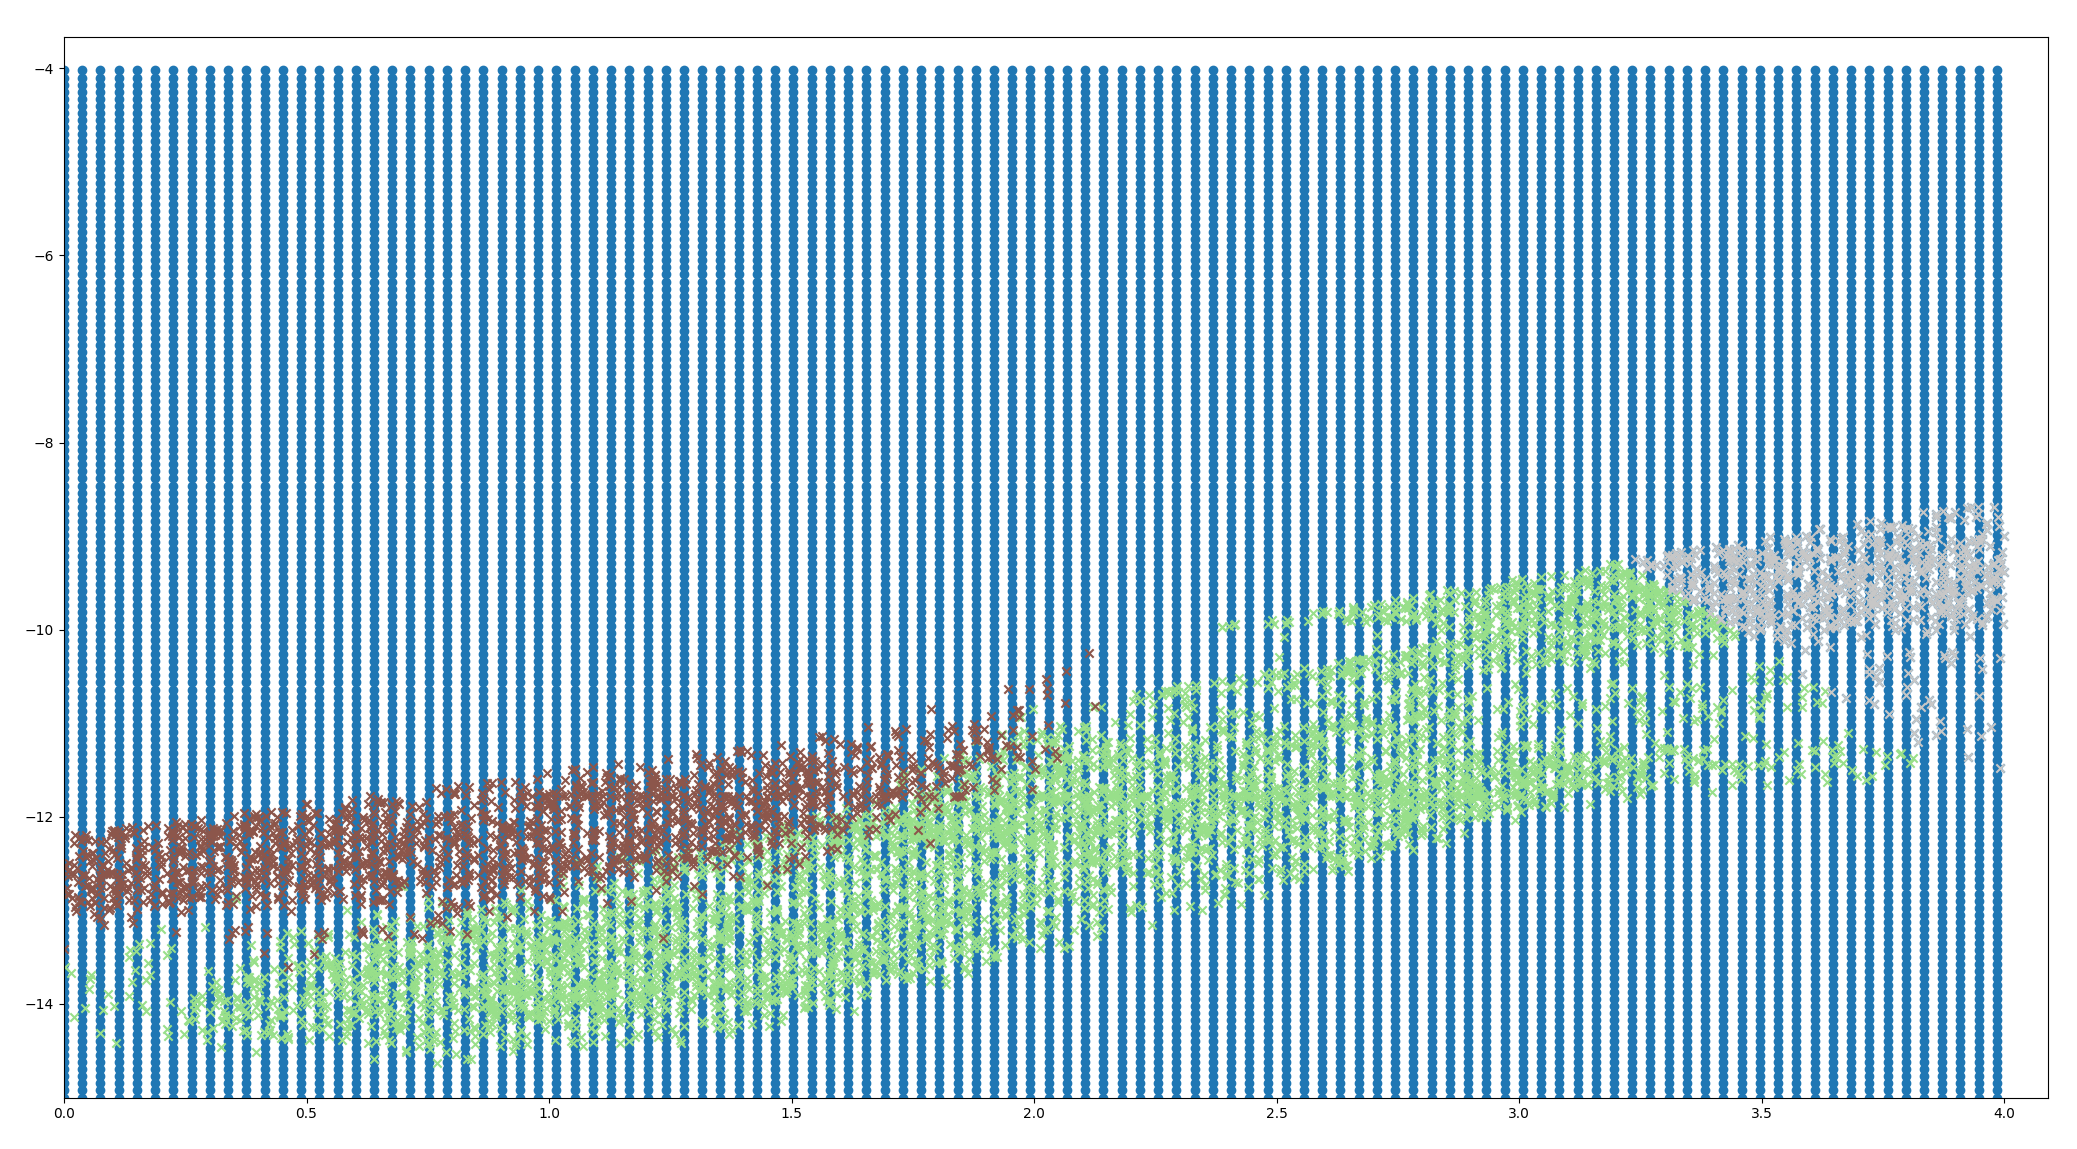
\includegraphics[width=0.8\textwidth]{separation-low-td-3-clusters}
    \caption{separation-low-td-3-clusters}
    \label{fig:separation-low-td-3-clusters}
\end{figure}

Now we try and exploit this, by making our splitting procedure check the TD
distance before settling in on a split. If it is lower than 0.95, we try and
increase the number of clusters. Then we look for the cluster with the largest
TD distance to the other clusters, and if this is large enough, we split the
region between that cluster and all the rest. For the region we looked at in
Figure~\ref{fig:separation-low-td-val}, that results in the wanted split, where
red points with the larger x-value are confined to their own region.

However, when the procedure repeats and gets back to remainder of the original
region where the clusters were overlapping, we get the result seen in
Figure~\ref{fig:overlap-3-clusters} when we make 3 clusters. Here, all 3
clusters have an overlap with one another.

\begin{figure}[ht]
    \centering
    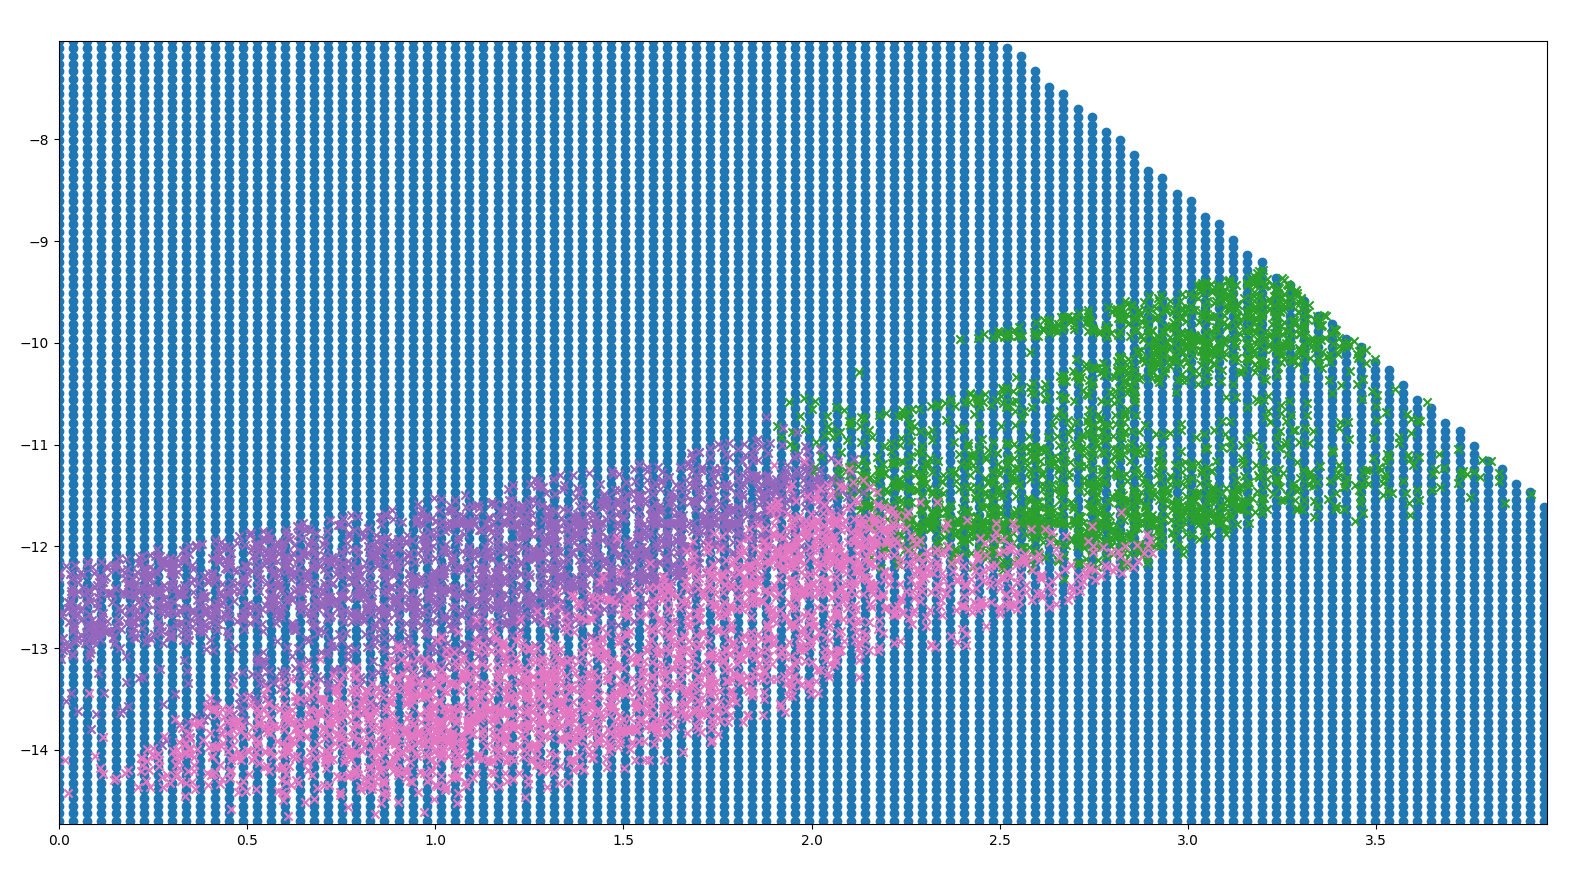
\includegraphics[width=0.8\textwidth]{overlap-3-clusters}
    \caption{%
        These 3 clusters are not perfectly separated. How to choose an
        appropriate split?
    }
    \label{fig:overlap-3-clusters}
\end{figure}

In Figure~\ref{fig:deterministic-stochastic-visualization} we show the same
region but where the points have been labelled according to wether their
transition probability vector assigns all probability to a single transition
(the red crosses) or spreads it accros multiple regions (the pink crosses). We
see 3 distinct areas, where the (sampled) transitions are deterministic and a
greater middle area with stochastic transitions.

\begin{figure}[ht]
    \centering
    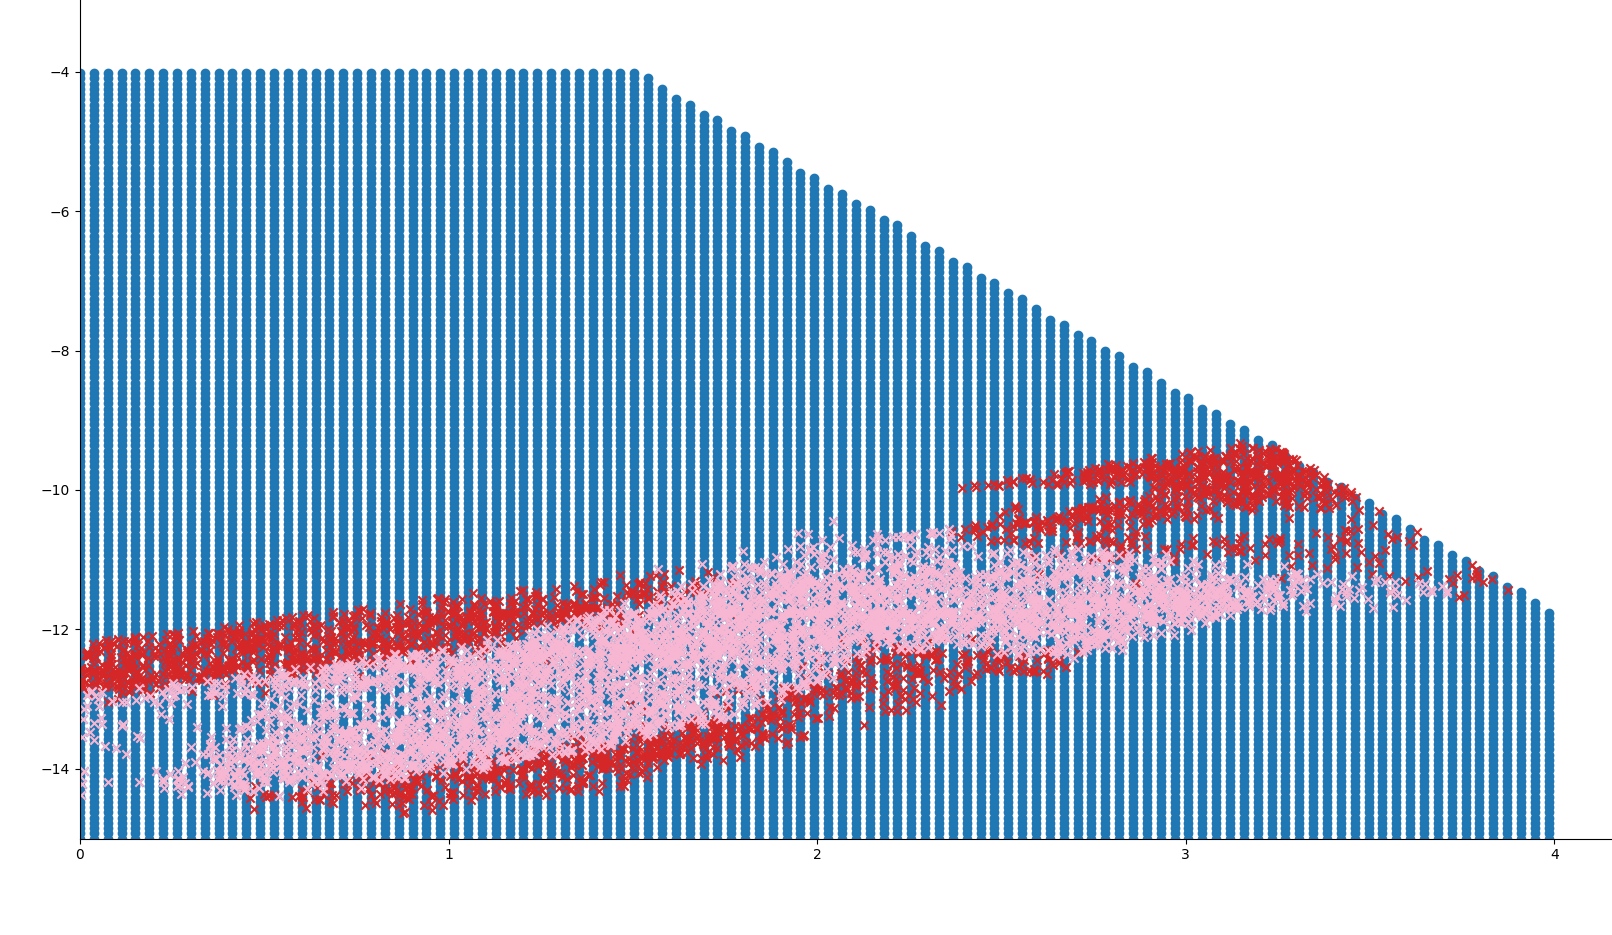
\includegraphics[width=0.8\textwidth]{deterministic-stochastic-visualization}
    \caption{%
        The red crosses are points with a probability vector assigning all
        probability on one transition. The pink crosses spreads the probability
        on multiple transitions.
    }
    \label{fig:deterministic-stochastic-visualization}
\end{figure}

\noindent
Ideas for how to separate these points (in
Figure~\ref{fig:deterministic-stochastic-visualization}):

\begin{itemize}
    \item Create 3 new regions, each characterized by the most probable
        transition. This would mean that each region is formed around the red
        points but contain the pink points whose transition probabilities are
        closest to those of the corresponding red points.
    \item Create 3 new regions that (almost) \textit{only} contain the red
        points and then another region containing the pink points; this would
        result in 3 regions with a very high certainty about the next region and
        then one region with a low certainty.
\end{itemize}

\section{Deterministic transitions}%
\label{sec:}

How do we separate regions where all states have deterministic transitions, but
there are 3 or more `groups' of transitions (ie.\ a group of states going to
region $x$, another to region $y$ and yet another to region $z$)? One idea is
simply to separate one group from all the other. However, if we look at an
example such as the one in Figure~\ref{fig:deterministic-groups1}, we see that
the choice of the group to split from the rest will have a pretty significant
impact on what kind of split can be made.

\begin{figure}[ht]
    \centering
    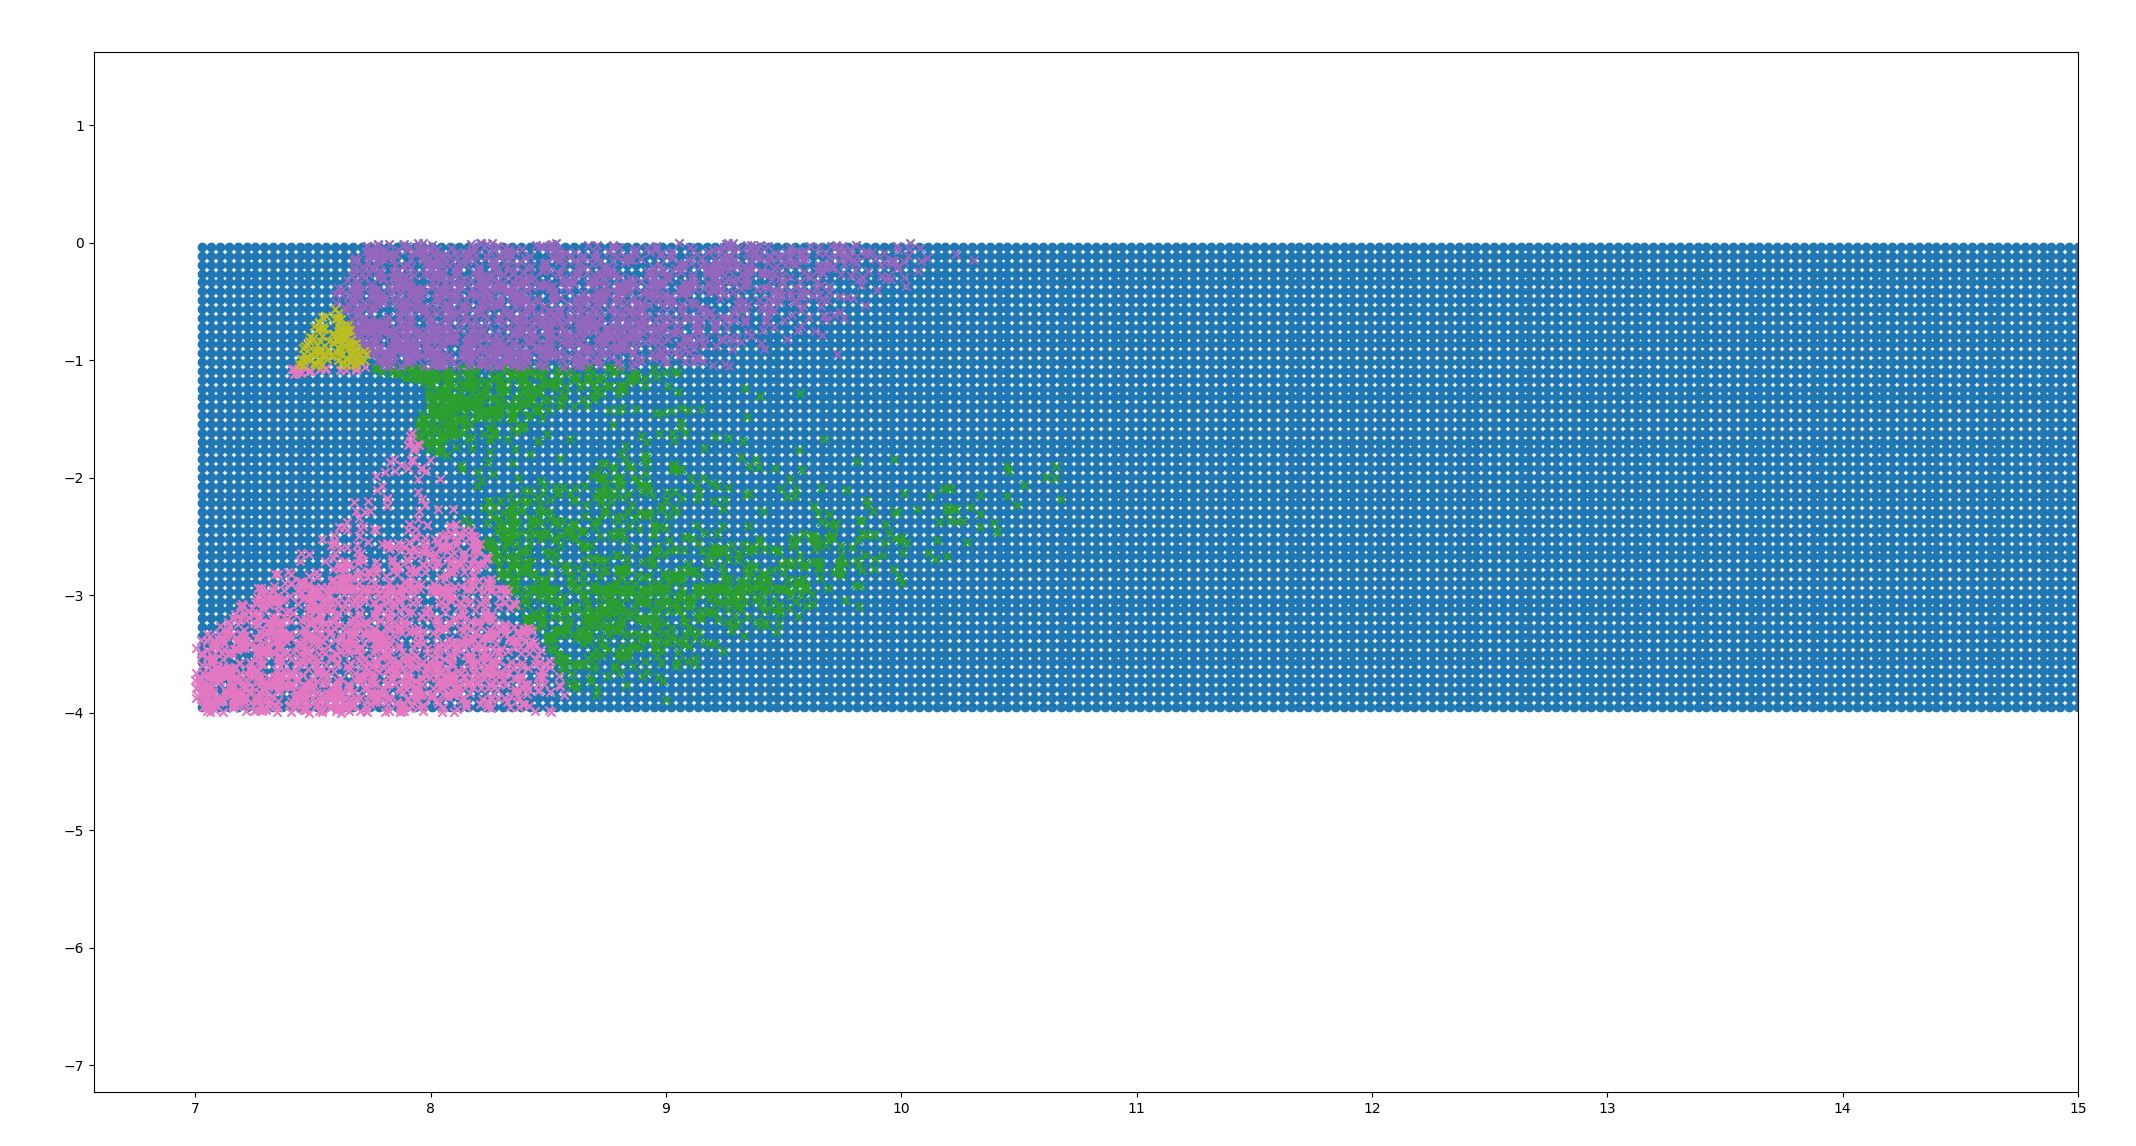
\includegraphics[width=0.8\textwidth]{deterministic-groups1}
    \caption{%
        Each color crosses represent a unique deterministic transition. As such,
        there are 4 groups of points in this region, each group transitioning
        with 100\% certainty to a specific next region.
    }
    \label{fig:deterministic-groups1}
\end{figure}

Whatever single group in Figure~\ref{fig:deterministic-groups1} we choose to split
from the rest, we would not be able to make an accurate split with a simple,
low-degree polynomial. However, it looks like we could separate the purple and
yellow groups from the green and pink groups by a nice linear boundary. As such,
the naive approach seems flawed. But how do we identify the good split? We could
test out all possible splits and select the one that has the best score balanced
with the lowest degree.

Another example of this is given in Figure~\ref{fig:deterministic-groups2}
and~\ref{fig:deterministic-groups2-split-with-2-clusters},
where we both see the discrete groups and the way they are split when using
aggloagglomorative clustering to separate 1 from the other.

\begin{figure}
    \centering
    \begin{subfigure}[ht]{0.9\textwidth}
        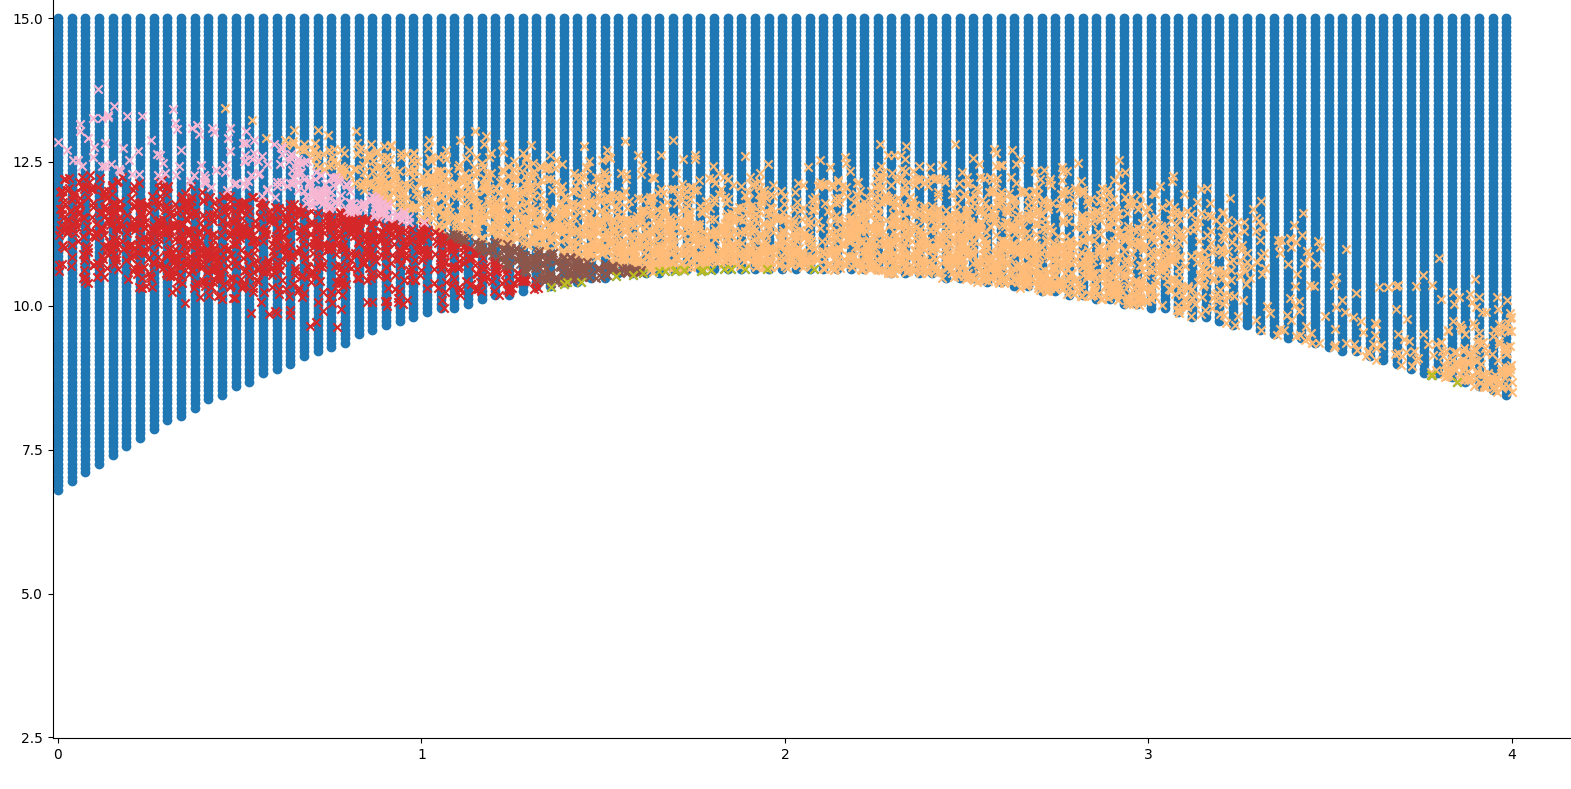
\includegraphics[width=\linewidth]{deterministic-groups2}
        \caption{Deterministic groups}%
        \label{fig:deterministic-groups2}
    \end{subfigure}
    \begin{subfigure}[ht]{0.9\textwidth}
        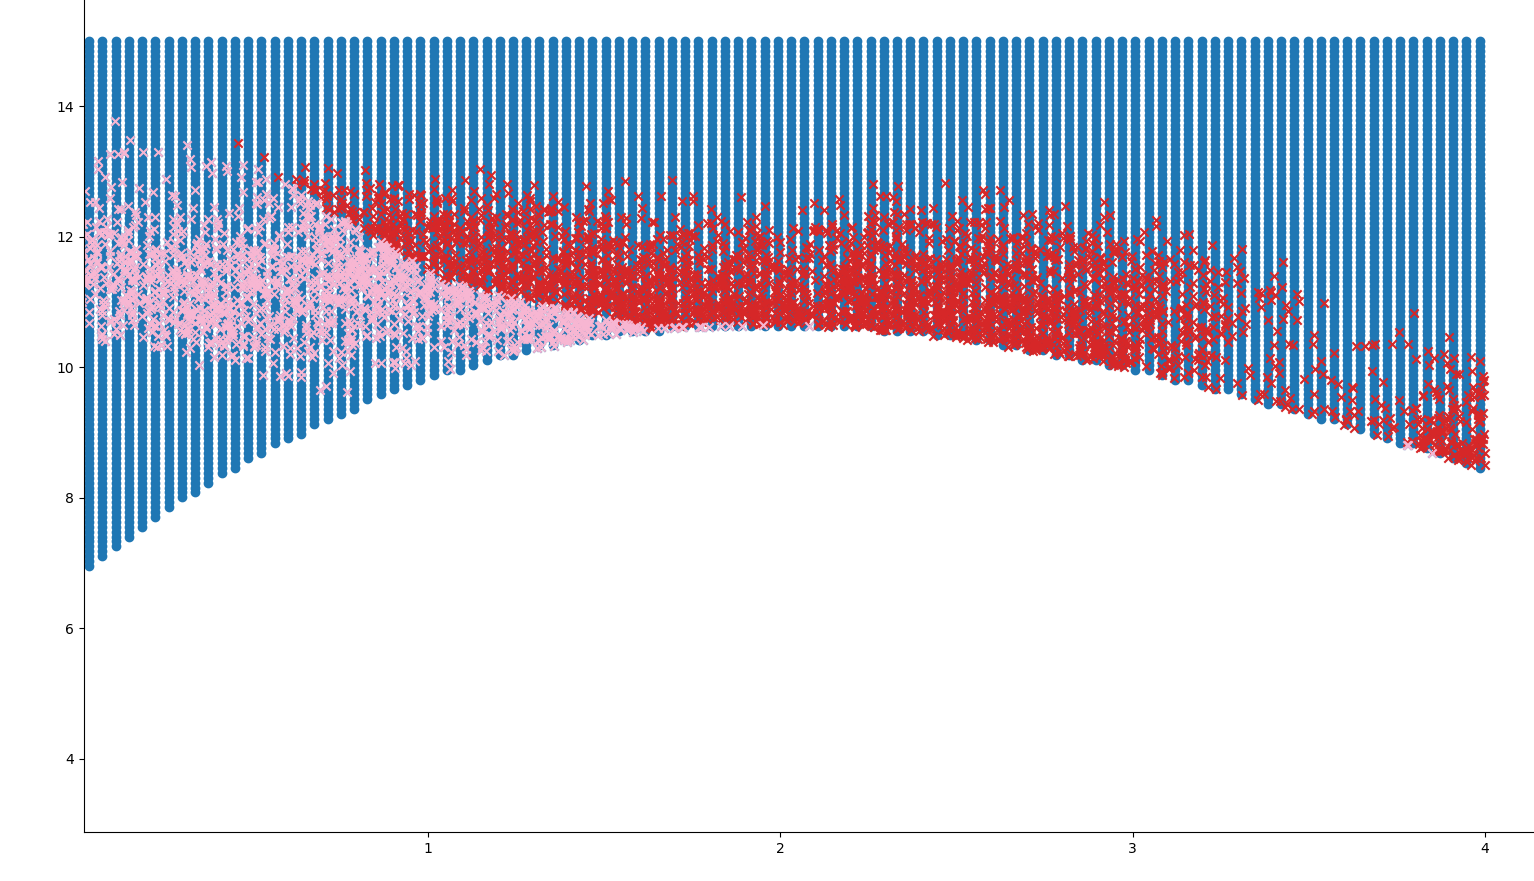
\includegraphics[width=\linewidth]{deterministic-groups2-split-with-2-clusters}
        \caption{2 splits}%
        \label{fig:deterministic-groups2-split-with-2-clusters}
    \end{subfigure}
    \caption{%
        Top: 5 distinct groups of deterministic transitions (yellow, pink,
        brown, red and green). Bottom: the split when just organising in 2
        clusters.
    }
    \label{fig:deterministic-groups2-full}
\end{figure}


In the next example, Figure~\ref{fig:deterministic-groups-misclassification1},
we have a more difficult situation, that harkens back to
Figure~\ref{fig:misclassification}. Here we have 3 groups of deterministic
transitions. However, one group (the grey one) is actually just a result of
misclassification. That is, these points `should' belong to a different region,
but since our splits inevitably are not 100\% accurate, we get these groups that
should actually not be considering when splitting. We want to ignore such
misclassified points and just consider them to belong to the group that they are
closest to in \textit{point-space} (in this case, the grey should belong to the
green group). But how do we identify this?

\begin{figure}[h!]
    \centering
    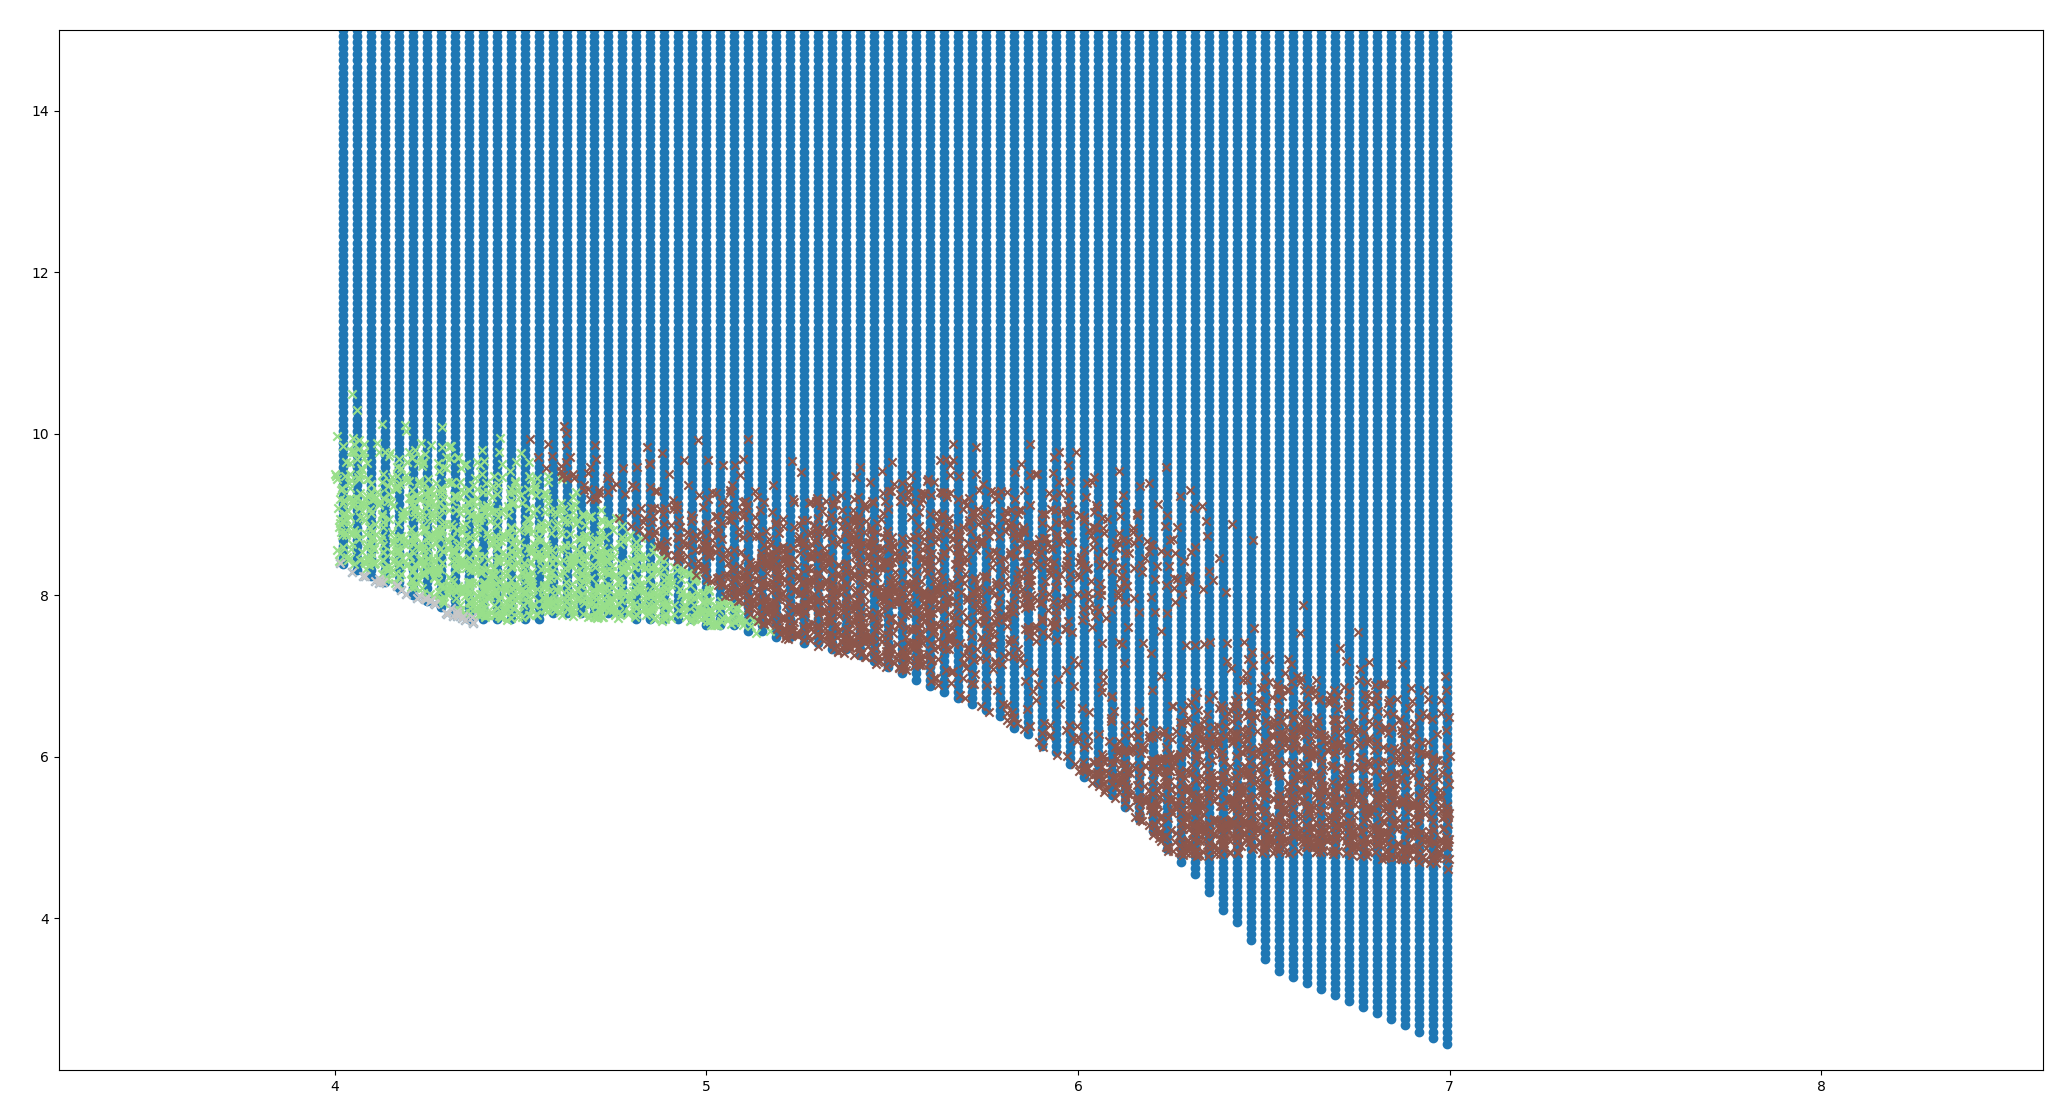
\includegraphics[width=0.8\textwidth]{deterministic-groups-misclassification1}
    \caption{fig:deterministic-groups-misclassification1}
    \label{fig:deterministic-groups-misclassification1}
\end{figure}

\subsubsection{Problem?}%

Imagine we have a 1-dimensional enviromnent, where a ball rolls along the
x-axis. At each timestep it will move a distance of 1 plus some gaussian noise
centered around 0. Can we partition this state space in such a way that it
meaningfully captures the behavior of the system? 

Let the dynamics of the system be such, that a ball observed in state $s^{t}$
will move a distance of $d \in [1 - a, 1 + a]$, where $a$ is some small positive
constant. We define a starting region $r^0 = \region[0]$ such that $\rmax[0] -
\rmin[0] = 1-a$ which ensures that whatever our initial state $s^0 \in r^0$, we
are guaranteed that $s^1$ will have left $r^0$.

We now know that $s^1$ will end up somewhere between $\rmin[0] + 1 - a$ and
$\rmax[0] + 1 + a$. If we use this to define the next region $r^1$, then we can
guarantee that for any $s^0 \in r^0$ we have that $s^1 \in r^1$. But we can't do
the same trick for $r^2$, since the domain of $s^2$ will be the range $[\rmin[0]
+ 2 - 2a, \rmax[0] + 2 + 2a]$. Since we defined $\rmax[0] - \rmin[0] = 1-a$ and
$a > 0$, we can see that 

\begin{align*}
    \rmin[0] + 2 - 2a &< \rmax[0] + 1 + a \\
    2 - 2a &< \rmax[0] - \rmin[0] + 1 + a \\
    2 - 2a &< 1 - a + 1 + a \\
    2 - 2a &< 2
\end{align*}

This means, that $s^2$ \textit{might} end up in $r^1$. Conversely, the upper
bound of the domain of $s^2$ is obviously larger than the upper bound of $r^1$
as we have $\rmax[0] + 2 + 2a > \rmax[0] + 1 + a$, meaning that $s^2$ might also
leave $r^1$. Therefore, we cannot for certain say what region states from $r^1$
will transition to --- and the only way to achieve this is by splitting $r^0$
into smaller regions thereby losing our guarentee of the transition function
from that region.

What if we define 2 sets of regions, $R_i$ and $R_j$, such that for all regions
$r^i \in R_i$ we have $\rmax[i] - \rmin[i] = 1-a$, and for all regions $r^j \in
R_j$ we have $\rmax[j] - \rmin[j] = (\rmax[i] + 1 + a) - (\rmin[i] + 1 - a) = 1
+ a$?\footnote{Note, in the following we will sometimes just write $r^j$ as a
shorthand for `a region $r \in R_j$'} Then for any region $r^i$, we know for
certain that the transitions will go to $r^{i+1} \in R_j$, and for any $r^j$, we
know that either $s^{t+1}$ stays in $r^j$ or $s^{t+1}$ transitions to a region
$r^{j+1} \in R_i$. More precisely, we know that in the range $[\rmin[j],
\rmin[j] + 2a]$ a state in $r^{j}$ \textit{may} stay in $r^j \in R_j$ and in the
range $[\rmin[j] + 2a, \rmax[j]]$ it will \textit{definitely} transition to
$r^{j+1} \in R_i$.

From this observation, consider the following: say we observe $\currstate$ in
$r^j \in R_j$. Then there are 2 possible regions for $\nextstate$, either $r^j
\in R_j$ or $r^{j+1} \in R_i$. However, given that we observed $\currstate$ in
$r^j$, we can now say with absolute certainty what the region of $\state[t+2]$
will be: if $\nextstate \in r^j$ then $\state[t+2] \in r^{j+1}$, and if
$\nextstate \in r^{j+1}$ then $\state[t+2] \in r^{j+2}$, where $r^{j+2} \in
R_j$. In other words, if the only thing we know about a state $\state$ is that
at time $t$ it was in $r^j \in R_j$ and we know what region it was in at time
$t+1$, then we know excactly what region it will be in at time $t+2$.

But what if $\currstate$ was in $r^i \in R_i$? Then we know that $\nextstate$ is
in $r^{i+1} \in R_j$ and then we just need to know the region at time $t+2$ to
determine (with certainty) the region at time $t+3$. This means, that by
observing 3 regions in a row (starting from a region in $R_i$), we can determine
the next region with absolute certainty. 

So, for a sequence of regions starting in $R_j$, we need just a sequence length
of 2 to determine the next region. If the sequence is starting in $R_i$, we need
3. But, if we observe $(r^j, r^i)$ then we might be able to determine that the
next region is $r^j$, but now we cannot know what will follow that, since we are
now stuck with a sequence of length 2 starting with $r^i$.

The possible region sequences are the following:

\begin{align*}
    &(r^i, r^j, r^i, r^j) \\
    &(r^i, r^j, r^j, r^i) \\
    &(r^j, r^i, r^j, r^i) \\
    &(r^j, r^i, r^j, r^j) \\
    &(r^j, r^j, r^i, r^j)
\end{align*}

% In this case, we need to think probabilistically. Does the expected value of
% $\nexstate$ depend on the region of $\currstate$? 

% We observe $\currstate \in r^j$ and lets say, that the probability of
% $\currstate$ taking any value in the range $\region[j]$ is uniform over that
% region. We then observe $r^i$. The probability that $\currstate$ transitioned to
% $r^i$ is 1 - the probability of staying in $r^j$. This in turn is equal to
% $(2a/1 + a) * $

\end{document}

